\title{Shioda's Modular Surface $S(5)$ and the Horrocks-Mumford Bundle}\label{chap2}
\markright{Shioda's Modular Surface $S(5)$ and the Horrocks-Mumford Bundle}

\author{By W.\@ Barth, K.\@ Hulek and R.\@ Moore}
\markboth{W. Barth, K. Hulek and R. Moore}{Shioda's Modular Surface $S(5)$ and the Horrocks-Mumford Bundle}

\date{}
\maketitle

\setcounter{page}{29}
\begin{figure}[H]
\centering
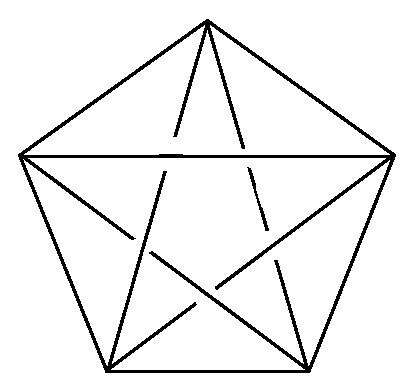
\includegraphics{figures/chap2-fig1.eps}
\end{figure}


\newpage



\setcounter{pageoriginal}{37}

\section{Introduction}\label{chap2-sec1}\pageoriginale


\subsection{Results and motivation}\label{chap2-sec1.1}


The Horrocks-Mumford bundle $\mathscr{F}$ on $\mathbb{P}_{4}$ was
discovered in 1972 and it is still essentially the only known
indecomposable rank-2 bundle on $\mathbb{P}_{4}$. Since 1972, all
efforts to construct more such bundles or to disprove their existence
have been in vain. In this situation, we believe it important to
understand better the bundle $\mathscr{F}$ itself. Our paper is a step
in this direction.

In this paper, we prove the following facts (see
section \ref{chap2-sec5.5}): The variety of {\em jumping lines} of
$\mathscr{F}$ is an {\em irreducible rational $4$-fold J.} The {\em
double} (or triple) {\em jumping lines} form a {\em surface
$J_{2}\subset J$.} Except for singularities along this surface the
4-fold $J$ is {\em smooth}.

The main tool in our study of the 4-fold $J$ is a birationally
equivalent smooth 4-fold $\widetilde{J}$, which in its turn is
constructed as the {\em blow-up of} $\mathbb{P}_{4}$ with respect to
the {\em ideal sheaf} of a singular surface $S_{15}$ of degree 15 in
$\mathbb{P}_{4}$. This surface $S_{15}$ is a copy of {\em Shioda's
elliptic modular surface} $S(5)$ immersed into $\mathbb{P}_{4}$ in
such a way that it acquires 30 double points, where two branches of
the surface meet.

The surface $S_{15}$ is (the closure of) the variety swept out by all
{\em quintic elliptic normal curves}, embedded $H_{5}$-{\em
equivariantly} in $\mathbb{P}_{4}$ for the Schroedinger action of the
Heisenberg group $H_{5}$ on $\mathbb{P}_{4}$. Alternatively $S_{15}$
can be described as the {\em determinantal locus} in $\mathbb{P}_{4}$
where the matrix of homogeneous polynomials
$$
\begin{pmatrix}
z^{2}_{0} & z^{2}_{1} & z^{2}_{2} & z^{2}_{3} & z^{2}_{4}\\[3pt]
z_{2}z_{3} & z_{3}z_{4} & z_{4}z_0 & z_{0}z_{1} & z_{1}z_{2}\\[3pt]
z_{1}z_{4} & z_{2}z_{0} & z_{3}z_{1} & z_{4}z_{2} & z_{0}z_{3}
\end{pmatrix}
$$\pageoriginale
drops its rank. Or $S_{15}$ can be considered as the image of the
surface $S(5)$ under the linear system $|I+2F|$, where $F$ is the
class of an elliptic fibre and $I$ is a divisor on $S(5)$ recentrly
considered in another context by Inoue and Livn\'e.

The systematic use of this surface $S_{15}$ is the basic new
achievement in our paper. Calculations which have been unaccessible so
far become practicable if one uses for appearing parameter points
$x\in \mathbb{P}_{4}$ the distinction, whether they lie outside of
$S_{15}$, on $S_{15}$ away from the 30 double points, or belong to the
double points. We study the properties of $S_{15}$ quite
carefully. This is motivated mainly by the following three reasons:
\begin{enumerate}
\item Elliptic quintic normal curves are mentioned in relation with
bundle $\mathscr{F}$ already in \cite{chap2-key6}. So the appearance
of the surface $S_{15}$ is quite natural. Totally unexpected for us
is, however, that Shioda's surface $S(5)$ is related to $\mathscr{F}$
in many more ways than the one given in this paper. In
sections \ref{chap2-sec1.2}, \ref{chap2-sec1.3} and \ref{chap2-sec1.4}
we describe what we know about this at present, but {\em were unable
to present with proofs in this paper} for the lack of time.

\item The divisor $I$ is interesting, because Inoue and Livn\'e use it
to construct a surface of general type with $c^{2}_{1}=3c_{2}$. Little
seems\pageoriginale to be known about the linear systems $|pI+qF|$,
$p$, $q\in \mathbb{N}$. Now some of them arise naturally in connection
with the Horrocks-Mumford bundle.

\item  Shioda's modular surface $S(n)$ exists for each
$n\in \mathbb{N}$, $n\geq 3$. The surface $S(3)$ is the blow up of
$\mathbb{P}_{2}$ in the 9 base points of the Hesse pencil. This is the
pencil of plane cubics invariant under the Heisenberg group
$H_{3}$. The surface $S(4)$ is swept out by all $H_{4}$-invariant
elliptic quartic normal curves in
$\mathbb{P}_{3}$. In \cite[p.~55]{chap2-key9} theta-functions are used
to identify the image in $\mathbb{P}_{3}$ as the Fermat quartic. There
it is also mentioned that similarly equations can be found defining
$S(n)$ for higher $n$. Our computations are related to properties of
theta-functions of level 5 in one variable. 
\end{enumerate}

\subsection{The surface \texorpdfstring{\boldmath$S_{25}$}{S25} (expository)}\label{chap2-sec1.2}

The smooth surface $S_{2p}\subset \mathbb{P}_{1}\times \mathbb{P}_{4}$
is introduced in section \ref{chap2-sec3.4}. We call it $S_{25}$,
because under the Segre map
$\mathbb{P}_{1}\times \mathbb{P}_{4}\to \mathbb{P}_{9}$ it goes to a
surface of degree 25 in $\mathbb{P}_{9}$. In fact this surface is the
complete intersection of Grass
$(\mathbb{P}_{1}\subset \mathbb{P}_{4})\subset \mathbb{P}_{9}$ with
the (suitably normalized) Segre variety
$\mathbb{P}_{1}\times \mathbb{P}_{4}\subset \mathbb{P}_{9}$. Notice
$\deg(\mathbb{P}_{1}\times \mathbb{P}_{4})=\deg \text{~Grass~}=5$. Alternatively
$S_{25}\subset\mathbb{P}_{9}$ can be described as the image of
Shioda's surface $S(5)$ under the complete linear system $|I+3F|$.

The surface $S_{25}$ enjoys a strange self-duality. In this way, it
para\-metrizes a 2-dimensional variety of planes in $\mathbb{P}_{4}$. It
turns out that these are the planes $Y_{v}$, $v\in S_{15}$
(see~\ref{chap2-sec5.1}) and that these are precisely the planes
$\mathbb{P}_{2}\subset \mathbb{P}_{4}$ on which the restricted bundle
$\mathscr{F}|\mathbb{P}_{2}$ is unstable. 

We\pageoriginale have $c_{1}(\mathscr{F}(-3))=-1$. If
$\mathscr{F}|\mathbb{P}_{2}$ is unstable for some plane
$\mathbb{P}_{2}\subset \mathbb{P}_{4}$, then
$\mathscr{F}(-3)|\mathbb{P}_{2}$ admits a unique section. This section
vanishes in four points. The four pencils of lines in $\mathbb{P}_{2}$
through these four points are the jumping lines in the plane. The six
lines connecting pairs among the four points are double jumping
lines.

Upon closer inspection, one finds that each double jumping line lies
in this way in three different planes.

\subsection{The surface of double jumping lines
(expository)}\label{chap2-sec1.3}

It is easy to see (cf.~5.2) that the only triple jumping lines are the
25 Horrocks-Mumford lines \cite[p.~72]{chap2-key6}
\begin{align*}
z_{k} &=
z_{k+2}+\epsilon^{j}z_{k+3}=z_{k+1}+\epsilon^{3j}z_{k+4}=0, j,
k=0,\ldots,4,\\
\epsilon &= e^{2\pi i/5}
\end{align*}
and that there are no jumping lines of order $\geq 4$. In this paper
we show that the double jumping lines are parametrized by a surface
$J_{2}\subset\text{~ Grass~ } (\mathbb{P}_{1}\subset \mathbb{P}_{4})$,
see section \ref{chap2-sec5.5}. There is a birational correspondence
between $J_{2}$ and the variety of sexti-secants of $S_{15}$. These
sexti-secants are separated in $\widetilde{J}$ after the blow up of
$S_{15}$. The birational map $\widetilde{J}\to J$ essentially consists
of blowing down the proper transforms of these sexti-secants. 

A ``generic'' surface in $\mathbb{P}_{4}$ should admit a finite number
of sexti-secants only. But $S_{15}$ comes with a two-dimensional
variety. They arise in two ways:
\begin{itemize}
\item[(a)] Joining\pageoriginale a point $P$ on a smooth fibre $E\subset S_{15}$
with $P'\in E$ such that $\mathscr{O}_{E}(P-P')$ is a 2-torsion class,
one obtains a secant of $S_{15}$. But this secant meets two more
smooth fibres in two other pairs of points differing by a 2-torsion
class and thus becomes a sexti-secant. The three fibres are related by
the fact that their quotients $E/$(2-torsion class) are isomorphic as
elliptic curves with level-5-structure.

\item[(b)] Shioda's surface $S(5)$ contains 25 sections $L_{i,j}$
differing by 5-torsion translations on the fibres and 25 3-sections
$C_{i,j}$ which consist of all the points differing from $L_{i,j}$ by
non-trivial 2-torsion translations on the fibres. It turns out that
the images of these curves $C_{i,j}$ on $S_{15}$ are plane sextics
(with six nodes). All lines in their 25 planes are sexti-secants. 
\end{itemize}

The sexti-secants of type (a) blown down parametrize the variety of
double jumping lines. The sexti-secants of type (b) blown down to 25
points parametrize the 25 triple jumping lines.

The curves $C_{i,j}$ are realizations of Bring's curve $C$. This is
the modular curve $\overline{\mathscr{H}/\Gamma_{0}(2,5)}$ where 
\begin{gather*}
H=\{z\in C:\text{~Im~}z>\phi\}\quad\text{is the upper
half-plane}\\[4pt]
\Gamma_{0}(2,5)=\left\{
\begin{pmatrix}
a & b\\[3pt]
c & d
\end{pmatrix}\in SL(2,Z):\begin{array}{l}a\equiv d\equiv 1(5)\\
b\equiv 0(5), c\equiv 0(10)\end{array}\right\}
\end{gather*}
There is a canonical $3:1$ map $C\to \mathbb{P}_{1}$ inducing a
rational $3:1$ map $\rho:S_{0}(2,5)\to S(5)$, where $S_{0}(2,5)$ is
Shioda's modular surface for the group $\Gamma_{0}(2,5)$. The fibres
of $S(5)$ are elliptic curves with level-5-structure (see~4.2),
whereas the fibres of $S_{0}(2,5)$\pageoriginale are elliptic curves with
level-5-structure and a distinguished non-trival 2-torsion
element. Forgetting this 2-torsion element is the $3:1$ map
$S_{0}(2,5)\to S(5)$.

So $S_{0}(2,5)$ birationally parametrizes pairs consisting of
sexti-secants of type (a) and of one of their six point of
intersection with $S_{15}$. The variety of sexti-secants themselves is
the image of $S_{0}(2,5)$ under the $6:1$ map
$$
S_{0}(2,5)\xrightarrow{\omega}S_{0}(2,5)\xrightarrow{\rho}S(5)
$$
where $\omega$ is the quotient map with respect to the distinguished
2-torsion translation on the fibres. Consequently, $J_{2}$ being
birationally equivalent to the variety of sexti-secants of type (a),
is birational to $S(5)$ again. In fact it is nothing but $S(5)$ with
its 25 sections blown down. The corresponding map $S(5)\to$ Grass
$(\mathbb{P}_{1}\subset \mathbb{P}_{4})\subset \mathbb{P}_{9}$ is
given by the linear system $|I+3F|$. So far this is the only linear
system $|pI+qF|$ on $S(5)$ where we know
$h^{0}(\mathscr{O}_{S(5)}(pI+qF))\neq 0$ and
$h^{1}(\mathscr{O}_{S(5)}(pI+qF))\neq 0$.

\subsection{The surface \texorpdfstring{\boldmath$S_{45}$}{S45}}\label{chap2-sec1.4}

If a plane varies in the family parametrized by $S_{25}$, so that the
restriction of $\mathscr{F}$ to the plane is unstable, the four points
in the plane, where the unique section violating stability vanishes,
describe a new surface $S_{45}$. Its degree turns out to be 45. Again
it is an image of Shioda's surface $S(5)$. This time the map is
rational, blowing up the 60 double points $P_{i}$ of singular fibres
on\pageoriginale $S(5)$ (see section \ref{chap2-sec4.3}). It is given
by the linear system $|3I+5F-\Sigma P_{i}|$.

Associating with a point on $S_{45}$ the (unique) unstable plane
containing it we obtain a rational $4:1$ map $S_{45}\to S_{25}$. This
is essentially the quotient map $S(5)\to S(5)$ with respect to the
four 2-torsion classes on the fibres.

A double jumping line is contained in three unstable planes and for
each one of these contains two points from $S_{45}$. Strangely enough
the double jumping lines being parametrized by sexti-secants of
$S_{15}$ are themselves sexti-secants of $S_{45}$.

\subsection{Notations and conventions}\label{chap2-sec1.5}

The base field will be $\mathbb{C}$ throughout this
paper. $\mathbb{P}_{n}$ will always denote
$\mathbb{P}_{n}(\mathbb{C})$, the $n$-dimensional complex-projective
space. $\mathbb{P}(V)$ is the space of lines in the vector space
$V$. If $v\in V$ is a non-zero vector, we denote by $v$ also the point
$\mathbb{C}v\in \mathbb{P}(V)$. We apologize in advance for using this
notation. But we believe that the context everywhere explains without
ambiguity whether a vector is meant or a point in projective
space. More generally, we even apply the following abuse of language:
We do not distinguish between a simple $p$-vector (i.e., an exterior
product $x_{1}\wedge\ldots\wedge x_{p}\in \wedge^{p}V$, $x_{i}\in V$
linearly independent), the vector space in $V$ spanned by
$x_{1},\ldots,x_{p}$, and the corresponding projective subspace in
$\mathbb{P}(V).\mathbb{Z}_{n}$ denotes the cyclic group of order $n$.

For $X\subset \mathbb{P}_{n}$, a subvariety with ideal sheaf
$\mathscr{I}_{x}\subset \mathscr{O}_{\mathbb{P}_{n}}$, we say
that\pageoriginale homogeneous polynomials $g_{1},\ldots,g_{k}$
describe $X$ schematically if $g_{1},\ldots,g_{k}$ generate
$\mathscr{I}_{x}$ at each point of $\mathbb{P}_{n}$

The first two authors are indebted to M.\@ Reid and D.\@ Burns for
stimulating and helpful conversations which were extremely useful for
this work.

\section{Some linear algebra}\label{chap2-sec2}

\subsection{Contraction and *-operators}\label{chap2-sec2.1}

Let $V$ be some $\mathbb{C}$-vector space of dimension $n$. (We are
interested only in the case $n=5$). An element in $\Lambda^{p}V$ is
called $p$-{\em vector}, and simple $p$-{\em vector} if it decomposes
as an exterior product $v_{1}\wedge\ldots\wedge v_{p}$, $v_{k}\in
V$. An element in $\Lambda^{p}V^{*}$ is called $p$-{\em form}. There
is the natural duality
$\Lambda^{p}V^{*}\otimes \Lambda^{p}V\to \mathbb{C}$ defined by 
$$
\langle h_{1}\wedge\ldots\wedge h_{p}, v_{1}\wedge\ldots,\wedge
v_{p}\rangle=\det (\langle h_{k},v_{l}\rangle), h_{k}\in V^{*},
v_{l}\in V.
$$
It extends to a {\em contraction map}
\begin{align*}
\Lambda^{p}V^{*}\otimes \Lambda^{q}V &\to 
\begin{cases}
\Lambda^{q-p}V & (p\leq q)\\[3pt]
\Lambda^{p-q}V^{*} & (p\geq q)
\end{cases}\\
g\otimes x &\to \langle g,x\rangle
\end{align*}
by
\begin{itemize}
\item[(1)] $\langle f,\langle g,x\rangle\rangle=\langle f\wedge
g,x\rangle$ for all $f\in \Lambda^{r}V^{*}(r=q-p\geq 0)$

\item[(2)] $\langle\langle g,x\rangle,y\rangle=\langle g,x\wedge
y\rangle$ for all $y\in \Lambda^{r}V(r=p-q\geq 0)$.

This\pageoriginale contraction is the adjoint operator to exterior
multiplication. One immediately checks formula (1) and (2) also for
all $r$, $0\leq r\leq q-p$, resp.\@ $0\leq r\leq p-q$. For $p=1$,
i.e., $h\in V^{*}$, and $x_{1},\ldots,x_{q}\in V$ we have

\item[(3)] $\langle h,x_{1}\wedge\ldots\wedge
x_{q}\rangle=\sum\limits^{q}_{k=1}(-1)^{q+k}\langle h,x_{k}\rangle
x_{1}\wedge\ldots \wedge \check{x}_{k} \wedge\ldots\wedge x_{q}$.

If $h\in V^{*}$, $x\in \Lambda^{q}V$ is arbitrary, then

\item[(4)] $\langle h,x\rangle=0\Leftrightarrow x\in \Lambda^{q}U$ with
$U=\ker h\subset V$.


Each basis $e_{1},\ldots,e_{n}\in V$ with dual basis
$\widehat{e}_{1},\ldots,\widehat{e}_{n}\in V^{*}$ induces isomorphisms
$\Lambda^{n}V\to \mathbb{C}$,
$x\to \langle \widehat{e}_{1}\wedge\ldots\wedge \widehat{e}_{n},x)$,
and $\Lambda^{n}V^{*}\to \mathbb{C}$, $g\to (g,e_{1}\wedge\ldots\wedge
e_{n}\rangle$. More generally we obtain isomorphisms
\begin{alignat*}{2}
&\Lambda^{p}V\to \Lambda^{n-p}V^{*}
&\qquad& \Lambda^{q}V^{*}\to \Lambda^{n-q}V\\
& x\to
x^{*}:=\langle \widehat{e}_{1}\wedge\ldots\wedge\widehat{e}_{n},x\rangle
&\qquad&
g\to g*=\langle g,e_{1}\wedge\ldots\wedge e_{n}\rangle
\end{alignat*}
satisfying as consequence of (1) and (2)

\item[(5)]
\begin{tabbing}
\= $\langle x^{*},y\rangle=(x\
y)^{*}(x\in \Lambda^{p}V,y\in \Lambda^{q}V,p+q\leq n)$\\[7pt]
\> $\langle f,g*\rangle=(f\wedge
g)*(f\in \Lambda^{p}V^{*},g\in \Lambda^{q}V^{*},p+q\leq n)$.
\end{tabbing}

These isomorphisms are each other's inverses \cite[\S\ 8.5,
prop.~4]{chap2-key4}, i.e., $(x^{*})*=x$ and $(f_{*})*=f$.
\end{itemize}

\setcounter{lemma}{0}
\begin{lemma}\label{chap2-lem1}
If\pageoriginale $n=5$, for all $x$, $y$, $z\in \Lambda^{2}V$ we have
\setcounter{equation}{5}
\begin{equation}
\langle (x\wedge y)^{*},z\rangle+\langle (y\wedge
z)^{*},x\rangle+\langle (z\wedge x)^{*},y\rangle=0\label{chap2-eq6}
\end{equation}
and in particular
\begin{equation}
\langle (x\wedge x)^{*},x\rangle=0\label{chap2-eq7}
\end{equation}
\end{lemma}

\begin{proof}
By linearity formula (6) needs to be verified for simple 2-vectors
$x=a_{1}\wedge a_{2}$, $y=a_{3}\wedge a_{4}$, $z=a_{5}\wedge a_{6}$
only. The whole expression (6) is multilinear in
$a_{1},\ldots,a_{6}$. From (3) it follows that it is alternating in
$a_{1},\ldots,a_{6}$. The assertion then is a consequence of
$\Lambda^{6}V=0$. 
\end{proof}

\subsection{The Horrocks-Mumford maps \texorpdfstring{\boldmath$f^{+}$}{f+} and
\texorpdfstring{$f^{-}$}{f-}}\label{chap2-sec2.2}

From now on, $V$ denotes a fixed copy of $\mathbb{C}^{5}$ with
standard basis $e_{0},\ldots,e_{4}$. We use the convention that
subscripts are elements of $\mathbb{Z}_{5}$, i.e., $e_{i+5}=e_{i}$. A
vector $v\in V$ is always written
$v=\sum\limits^{4}_{0}v_{i}e_{i}$. In \cite{chap2-key6} the two maps
$f^{\pm}:V\to \Lambda^{2}V$
$$
f^{+}(v)=\sum v_{i}e_{i+2}\wedge e_{i+3}\quad f^{-}(v)=\sum
v_{i}e_{i+1}\wedge e_{i+4}
$$
are introduced. In addition, we use the following abbreviations
\begin{align*}
& h^{+}(v):=\sfrac{1}{2}(f^{+}(v)\wedge f^{+}(v))^{*}=\sum
v_{i+1}v_{i+4}\widehat{e}_{i}\\
& h^{-}(v):=\sfrac{1}{2}(f^{-}(v)\wedge f^{-}(v))^{*}=-\sum
v_{i+2}v_{i+3}\widehat{e}_{i}\\
& h^{\circ}(v):=(f^{+}(v)\wedge f^{-}(v))^{*}=\sum
v^{2}_{i}\widehat{e}_{t}\\
& v^{+}=v^{+}(v):=-\langle h^{\circ}(v),f^{+}(v)\rangle
=(\sum(v_{i+2}v^{2}_{i+4}-v^{2}_{i-1}v_{i+3})e_{i}\\
& v^{-}=v^{-}(v):=-\langle h^{\circ}(v),f^{-}(v)\rangle =\sum (v_{i+1}v^{2}_{i+2}-v^{2}_{i+3}v_{i+4})e_{i}
\end{align*}\pageoriginale

We observe
\begin{equation*}
h^{\circ}(v)\neq 0\quad\text{for all}\quad 0\neq v\in V.\tag{8}
\end{equation*}

As a consequence of (6) and (7), we find
\begin{equation*}
\begin{split}
& \langle h^{-}(v),f^{+}(v)\rangle =\langle\sfrac{1}{2}(f^{-}\wedge
f^{-})^{*},f^{+}\rangle=-\langle (f^{+}\wedge f^{-})^{*},f^{-}>=v\\
& \langle h^{+}(v),f^{-}(v)\rangle =\langle \sfrac{1}{2}(f^{+}\wedge
f^{+})^{*},f^{-}\rangle =-\langle (f^{+}\wedge f^{-})^{*},f^{+}\rangle
=v^{+}\\
& \langle h^{+}(v),f^{+}(v)\rangle =\langle \sfrac{1}{2}(f^{+}\wedge f^{+})^{*},f^{+})=0\\
& \langle h^{-}(v),f^{-}(v)\rangle =\langle \sfrac{1}{2}(f^{-}\wedge
f^{-})^{*},f^{-}\rangle =0
\end{split}\tag{9}
\end{equation*}

Using this and (1), we get
\begin{equation*}
\begin{split}
\langle h^{\circ}(v),v^{\pm}\rangle &= -\langle h^{\circ},\langle
h^{\circ},f^{\pm}\rangle\rangle =-\langle h^{\circ}\wedge
h^{\circ},f^{\pm}\rangle=0\\
\langle h^{+}(v),v^{+}\rangle &= \langle h^{+},\langle
h^{+},f^{-}\rangle\rangle=\langle h\wedge h^{+},f^{-}\rangle =0\\
\langle h^{+}(v),v^{-}\rangle &= -\langle h^{+},\langle
h^{\circ},f^{-}\rangle\rangle=-\langle h^{+}\wedge
h^{\circ},f^{-}\rangle\\
&= \langle h^{\circ},\langle h^{+},f^{-}\rangle\rangle=\langle
h^{\circ},v^{+}\rangle=0\\
\langle h^{-}(v),v^{-}\rangle &= \langle
h^{-}(v),v^{+}\rangle=0\quad\text{similarly.}  
\end{split}
\tag{10}
\end{equation*}
The\pageoriginale exterior products of the forms $h^{+}(v)$,
$h^{\circ}(v)$, $h^{-}(v)$ are given by
\begin{align*}
(h^{\circ}(v)\wedge h^{\pm}(v))_{*} &= \sfrac{1}{2}\langle
h^{\circ},f^{\pm}\wedge f^{\pm}\rangle\tag{5}\\
&= \langle h^{\circ},f^{\pm}\rangle\wedge f^{\pm}\tag{3}\\
&= -v^{\pm}\wedge f^{\pm}(v)
\end{align*}

\begin{itemize}
\item[(11)]
\begin{align*}
(h^{+}(v)\wedge h^{-}(v))_{*} &= \sfrac{1}{2}(h^{+},f^{-}\wedge f^{-})\tag{5}\\
&= \langle h^{+},f^{-}\rangle \wedge f^{-}\tag{3}\\
&=v^{+}\wedge f^{-}(v)=-v^{-}\wedge f^{+}(v)\\
(h^{+}(v)\wedge h^{-}(v)\wedge h^{\circ}(v))_{*} &= -((v^{-}\wedge
f^{+})^{*}\wedge h^{\circ})_{*}\\
&= \langle h^{\circ},v^{-}\wedge f^{+}\rangle\tag{5}\\
&= \langle h^{\circ},v^{-}\rangle f^{+}+v^{-}\wedge \langle
h^{\circ},f^{+}\rangle \tag{3}\\
&= v^{+}\wedge v^{-}
\end{align*}
\end{itemize}

\subsection{The condition \texorpdfstring{\boldmath$v^{+}=v^{-}=0$}{v0}.}\label{chap2-sec2.3}

The next proposition gives several descriptions of the set $\{v\in
V:v^{+}=v^{-}=0\}$. 

\begin{proposition}\label{chap2-prop1}
For\pageoriginale $v\in V$, the following properties are equivalent.
\begin{itemize}
\item[\rm(i)] $v^{+}=v^{-}=0$

\item[\rm(ii)] $h^{+}(v)$, $h^{\circ}(v)$ and $h^{-}(v)$ are
proportional

\item[\rm(iii)] $\lambda f^{+}(v)+\mu f^{-}(v)$ is a simple bivector
for two different ratios $(\lambda:\mu)\in \mathbb{P}_{1}$

\item[\rm(iv)] $v$ is a multiple of one of the 30 vectors
\begin{align*}
& e_{k}, k=0,\ldots,4\\
& e_{kl}=(1,\epsilon^{k+1},\epsilon^{2k+3l},\epsilon^{4k})k,
l=0,\ldots,4,\epsilon=e^{2\pi i/5}
\end{align*}
\end{itemize}
\end{proposition}

\begin{proof}
\begin{description}
\item[iii) $\Rightarrow$ ii):]
By assumption, there are two different $(\lambda:\mu)\in\mathbb{P}_{1}$ with $\lambda^{2}h^{+}(v)+\lambda\mu h^{\circ}(v)+\mu^{2}h^{-}(v)=0$. This implies that the forms $h^{+}(v)$, $h^{\circ}(v)$, $h^{-}(v)$ span a space of dimension 1.

\item[ii) $\Rightarrow$ i):]
By (11), we have $v^{+}\wedge f^{\pm}(v)=v^{-}\wedge f^{\pm}(v)=0$. If
$v^{+}\neq 0$ or $v^{-}\neq 0$, this leads to $f^{+}(v)\wedge
f^{-}(v)=0$, in conflict with (8). 
 
\item[i) $\Rightarrow$ iv):]
The assumption is
\begin{alignat*}{2}
& v_{2}v^{2}_{4}=v^{2}_{1}v_{3} &\qquad&
v_{1}v^{2}_{2}=v^{2}_{3}v_{4}\\
& v_{3}v^{2}_{0}=v^{2}_{2}v_{4} &\qquad&
v_{2}v^{2}_{3}=v^{2}_{4}v_{0}\\
& v_{4}v^{2}_{1}=v^{2}_{3}v_{0} &\qquad&
v_{3}v^{2}_{4}=v^{2}_{0}v_{1}\\
& v_{0}v^{2}_{2}=v^{2}_{4}v_{1} &\qquad&
v_{4}v_{0}^{2}=v^{2}_{1}v_{2}\\
& v_{1}v^{2}_{3}=v^{2}_{0}v_{2} &\qquad& v_{0}v^{2}_{1}=v^{2}_{2}v_{3} 
\end{alignat*}
\end{description}

We\pageoriginale distinguish between two cases:

\begin{description}
\item[Case 1.] One of the coordinates $v_{i}$ vanishes. By $(i\to
i+1)$-symmetry we may assume $v_{0}=0$. The equations then are
equivalent with
$$
v_{i}v_{j}=0\quad\text{for all}\quad 1\leq i\neq j\leq 4.
$$
So all coordinates but one vanish.

\item[Case 2.] $v_{i}\neq 0$ for all $i$. We may put
$$
v_{0}=1, \ v_{1}=\alpha\beta, \ v_{2}=\alpha^{2}\beta^{3},
$$
and find the equations equivalent with
$$
v_{3}=\alpha^{-2}\beta^{-4}, \
v_{4}=\alpha^{4}\beta^{5}, \ \alpha^{5}=\beta^{5}=1. 
$$
Putting $\alpha=\epsilon^{k}$, $\beta=\epsilon^{l}$ we obtain
$v=e_{kl}$.

\item[iv) $\Rightarrow$ iii):] if $v=e_{k}$, then
$h^{+}(v)=h^{-}(v)=0$ and $f^{\pm}(v)$ both are simple bivectors. if
$v=e_{kl}$, then
\begin{align*}
&
h^{\circ}(e_{kl})=\widehat{e}_{0}+\epsilon^{2k+2l}\widehat{e}_{1}+\epsilon^{4k+1}\widehat{e}_{2}+\epsilon^{4+2l}\widehat{e}_{3}+\epsilon^{3k}\widehat{e}_{4}\\
& h^{+}(e_{kl})=\epsilon^{l}h^{0}(e_{kl}),\quad
h^{-}(e_{kl})=-\epsilon^{-l}h^{\circ}(e_{kl}) 
\end{align*}
show that
$$
\lambda^{2}h^{+}(e_{kl})+\lambda\mu
h^{\circ}(e_{kl})+\mu^{2}h^{-}(e_{kl}) 
$$
vanishes\pageoriginale if and only if
$$
\epsilon^{l}\lambda^{2}+\lambda\mu-\epsilon^{-l}\mu^{2}=0.
$$
This quadratic polynomial has the two different roots
\item[(12)]
$\lambda/\mu=-\epsilon^{-l}(1\pm \sqrt{5})/2$,

corresponding to simple bivectors $\lambda f^{+}(e_{kl})+\mu f^{-}(e_{kl})$.
\end{description}
\end{proof}

We shall need explicitly the polynomial
$$
f(\lambda,\mu)=\prod^{4}_{l=0}\left(\epsilon^{l}\lambda^{2}+\lambda\mu-\epsilon^{-l}\mu^{2}\right)
$$
which has the 10 roots (12.) Obviously
\begin{align*}
f(\epsilon \lambda,\mu) &
=\Pi \epsilon^{l+2}\lambda^{2}+\epsilon\lambda\mu-\epsilon^{-l}\mu^{2}\\
&=\Pi \epsilon(\epsilon^{l+1}\lambda^{2}+\lambda\mu-\epsilon^{-l-1}\mu^{2})\\
&= f(\lambda,\mu)
\end{align*}
and similarly $f(\lambda,\epsilon\mu)=f(\lambda,\mu)$. This shows
$$
f(\lambda,\mu)=a\lambda^{10}+b\lambda^{5}\mu^{5}+c\mu^{10}
$$

We have
\begin{align*}
a&
=1\cdot \epsilon \cdot \epsilon^{2}\cdot \epsilon^{3}\cdot \epsilon^{4}=1\\
c& =(-1)(-\epsilon)(-\epsilon^{2})(-\epsilon^{3})(-\epsilon^{4})=-1\\
b&= f(1,1)\\
 &=
 (\epsilon+1-\epsilon^{4})(\epsilon^{2}+1-\epsilon^{3})(\epsilon^{3}+1-\epsilon^{2})(\epsilon^{4}+1-\epsilon)\\
&= 11 
\end{align*}
\pageoriginale

\begin{description}
\item[(13)] $f(\lambda,\mu)=\lambda^{10}+11\lambda^{5}\mu^{5}-\mu^{10}$
\end{description}

\subsection{The condition \texorpdfstring{\boldmath$v^{+}\wedge v^{-}=0$}{v+}.}\label{chap2-sec2.4}

The next proposition gives several descriptions of the set $\{v\in
V:v^{+}(v)\wedge v^{-}(v)=0\}$.

\begin{proposition}\label{chap2-prop2}
The following conditions on $v\in V$ are equivalent:
\begin{itemize}
\item[\rm(i)] $v^{+}\wedge v^{-}=0$

\item[\rm(ii)] $h^{+}(v)\wedge h^{\circ}(v)\wedge h^{-}(v)=0$

\item[\rm(iii)] from some $(\lambda,\mu)\in \mathbb{C}^{2}\backslash
0:\lambda v^{+}-\mu v^{-}=0$

\item[\rm(iv)] from some $(\lambda,\mu)\in \mathbb{C}^{2}\backslash 0$
$$
\lambda^{2}h^{+}(v)+\lambda \mu h^{\circ}(v)+\mu^{2}h^{-}(v)=0
$$

\item[\rm(v)] for some $(\lambda,\mu)\in \mathbb{C}^{2}\backslash
0:\lambda f^{+}(v)+\mu f^{-}(v)$ is a simple bivector.
\end{itemize}
Unless $v^{+}=v^{-}=0$, the ratio $(\lambda:\mu)\in \mathbb{P}_{1}$ is
uniquely determined by {\rm (iii), (iv),} or {\rm (v)} and is the same
in all three equations.
\end{proposition}

\begin{proof}
Properties\pageoriginale (i) and (ii) are equivalent by (11). Properties (i) and
(iii) are obviously equivalent, and (iv) obviously implies
(ii). Properties (iv) and (v) (with the same $(\lambda:\mu)$) are
equivalent by definition of $h^{+}$, $h^{\circ}$, $h^{-}$.

To show the direction (ii) $\Rightarrow$ (iv), we assume
$$
c^{+}h^{+}(v)+c^{\circ}h^{\circ}(v)+c^{-}h^{-}(v)=0,
(c^{\pm},c^{\circ})\in \mathbb{C}^{3}\backslash 0.
$$
Contracting this equation with $f^{\pm}(v)$ and using (9) we find 
$$
-c^{\circ}v^{+}+c^{-}v^{-}=c^{+}v^{+}-c^{\circ}v^{-}=0.
$$
The case $v^{+}=v^{-}=0$ being settled by
proposition \ref{chap2-prop1} we may assume $v^{+}\neq 0$ or
$v^{-}\neq 0$. Taking $(\lambda,\mu)\neq (0,0)$ as in (iii), we find
\begin{align*}
c^{\circ}\mu-c^{-}\lambda &= c^{+}\mu-c^{\circ}\lambda=0\\[3pt]
(c^{\circ})^{2} &= c^{+}c^{-}
\end{align*}
So there is $(\lambda',\mu')\in \mathbb{C}^{2}\backslash 0$ with
$c^{+}=(\lambda)2$, $c^{\circ}=\lambda'\mu'$, $c^{-}=(\mu')^{2}$. This
proves (iv). Additionally we observe that $(\lambda,\mu)$ and
$(\lambda',\mu')$ are proportional.
\end{proof}

If $\lambda f^{+}(v)+\mu f^{-}(v)$ is a simple bivector, it describes
some 2-dimensio\-nal vector space in $V$. The vector
$$
-\langle h^{\circ}(v), \lambda f^{+}(v)+\mu f^{-}(v)\rangle =\lambda
 v^{+}+\mu v^{-}
$$
spans the intersection of this space with the hyperplane $\{u:\langle
h^{\circ}(v),u\rangle=0\}$, unless $v^{+}=v^{-}=0$.

We\pageoriginale observe
\begin{itemize}
\item[(14)] $v^{\pm}\wedge (\lambda f^{+}(v)+\mu f^{-}(v))=0$

whenever $\lambda f^{+}(v)+\mu f^{-}(v)$ is simple.
\end{itemize}

\subsection{The curves \texorpdfstring{$E_{\lambda:\mu}$}{El}}\label{chap2-sec2.5}

We denote by $E_{\lambda:\mu}\subset \mathbb{P}_{4}(V)$ the set
described by vectors $v$ such that $\lambda f^{+}(v)+\mu f^{-}(v)$ is
simple. It was shown (proposition \ref{chap2-prop2}
in \ref{chap2-sec2.4}) that for two different ratios $(\lambda:\mu)$
the two sets $E_{\lambda:\mu}$ are disjoint, unless the ratios are
$0$, $\infty$ or two from the 10 ones in (12) differing by the
sign. By proposition \ref{chap2-prop2} (iv) we have the following
quadratic equations for this set
\setcounter{equation}{14}
\begin{equation}
\begin{split}
& Q_{0}(\lambda,\mu)=\lambda^{2}v_{1}v_{4}+\lambda \mu
v^{2}_{0}-\mu^{2}v_{2}v_{3}=0\\
& Q_{1}(\lambda,\mu)=\lambda^{2}v_{2}v_{0}+\lambda \mu
v^{2}_{1}-\mu^{2}v_{3}v_{4}=0\\
& Q_{2}(\lambda,\mu)=\lambda^{2}v_{3}v_{1}+\lambda \mu
v^{2}_{2}-\mu^{2}v_{4}v_{0}=0\\
& Q_{3}(\lambda,\mu)=\lambda^{2}v_{4}v_{2}+\lambda\mu
v^{2}_{3}-\mu^{2}v_{0}v_{1}=0\\
& Q_{4}(\lambda,\mu)=\lambda^{2}v_{0}v_{3}+\lambda\mu
v^{2}_{4}-\mu^{2}v_{1}v_{2}=0 
\end{split}\label{chap2-eq15}
\end{equation}

\begin{proposition}\label{chap2-prop3}
The subscheme $E_{\lambda:\mu}\subset \mathbb{P}_{4}$ given by
equations \eqref{chap2-eq15} is a smooth curve unless
$\lambda\backslash \mu$ takes one of the following 12 values:
$$
0,\infty, -\epsilon^{-l}(1\pm \sqrt{5})/2 \quad (l=0,\ldots,4)
$$
\end{proposition}

\begin{proof}
We\pageoriginale show that the matrix of partial derivatives
$\partial_{i}Q_{j}(\lambda,\mu)$
$$
\begin{pmatrix}
2\lambda \mu v_{0} & \lambda^{2}v_{2} & -\mu^{2}v_{4} & -\mu^{2}v_{1}
& \lambda^{2}v_{3}\\
\lambda^{2}v_{4} & 2\lambda \mu v_{1} & \lambda^{2}v_{3} &
-\mu^{2}v_{0} & -\mu^{2}v\\
-\mu^{2}v_{3} & \lambda^{2}v_{0} & 2\lambda\mu v_{2}
& \lambda^{2}v_{4} & -\mu^{2}v_{1}\\
-\mu^{2}v_{2} & -\mu^{2}v_{4} & \lambda^{2}v_{1} & 2\lambda \mu v_{3}
& \lambda^{2}v_{0}\\
\lambda^{2}v_{1} & -\mu^{2}v_{3} & -\mu^{2}v_{0} & \lambda^{2}v_{2} &
2\lambda \mu v_{4}
\end{pmatrix}
$$
has rank $\geq 3$, unless $(\lambda:\mu)$ is one of the 12 special
parameters above. We denote by $\det^{ijk}_{lmn}$ the $3\times
3$-subdeterminant in the rows $l$, $m$, $n$ and columns $i$, $j$, $k$
and compute
\begin{align*}
\det\nolimits^{i,i+1,i+4}_{i,i+1,i+4}
&= \lambda \{8\lambda^{2}\mu^{3}v_{t}v_{i}v_{i+1}v_{i+4}-2\mu^{5}v_{i}v_{i+2}v_{i+3}\\
&\quad -2\lambda^{4}\mu(v_{i+2}v^{2}_{i+4}+v^{2}_{i+1}v_{i+3})
 -\lambda^{3}\mu^{2}(v_{i+1}v^{2}_{i+2}+v^{2}_{i+3}v_{i+4})\}\\
\det\nolimits^{i,i+2,i+3}_{i,i+2,i+3}&= \mu\{-2\lambda^{5}v_{i}v_{i+1}v_{i+4}+8\lambda^{3}\mu^{2}v_{i}v_{i+2}v_{i+3})\\
&\quad +\lambda^{2}\mu^{3}(v_{i+2}v^{2}_{i+4}+v^{2}_{i+1}v_{i+3})
 -2\lambda \mu^{4}(v_{i+1}v^{2}_{i+2}+v^{2}_{i+3}v_{i+4})\}\\
\det\nolimits^{i,i+1,i+4}_{i,i+2,i+3}
&=\mu \{-2\lambda \mu^{4}v_{i}v_{i+1}v_{i+4}+2\lambda^{5}v^{3}_{i}+2\lambda^{4}\mu
v_{i}v_{i+2}v_{i+3}\\
&\quad +\lambda^{2}\mu^{3}(v_{i+1}v^{2}_{i+2}+v^{2}_{i+3}v_{i+4})\}\\
\det\nolimits^{i,i+2,i+3}_{i,i+1,i+4}
&= \lambda \{2\lambda \mu^{4}v_{i}v_{i+1}v_{i+4}-2\mu^{5}v^{3}_{i}+2\lambda^{4}\mu
v_{i+2}v_{i+3}\\
&\quad +\lambda^{3}\mu^{2}(v_{i+2}v^{2}_{i+4}+v^{2}_{i+1}v_{i+3})\}
\end{align*}\pageoriginale
We may assume $\lambda \mu \neq 0$. Let $v\in E_{\lambda:\mu}$ be some
point where the matrix $(\partial_{i}Q_{j}(\lambda,\mu))$ has rank
$\leq 2$. Then
$$
\begin{pmatrix}
8\lambda^{2}\mu^{3} & 0 & -2\mu^{5} & -2\lambda^{4}\mu &
-\lambda^{3}\mu^{2}\\[5pt]
-2\lambda^{5} & 0 & 8\lambda^{3}\mu^{2} & \lambda^{2}\mu^{3} &
-2\lambda \mu^{4}\\[5pt]
-2\lambda \mu^{4} & 2\lambda^{5} & 2\lambda^{4}\mu & 0
& \lambda^{2}\mu^{3}\\[5pt]
2\lambda\mu^{4} & -2\mu^{5} & 2\lambda^{4}\mu & \lambda^{3}\mu^{2} & 0
\end{pmatrix}
\begin{pmatrix}
v_{i}v_{i+1}v_{i+4}\\[5pt]
v^{3}_{i}\\[5pt]
v_{i}v_{i+2}v_{i+3}\\[5pt]
v_{i+2}v^{2}_{i+4}+v^{2}_{i+1}v_{i+3}\\[5pt]
v_{i+1}v^{2}_{i+2}+v^{2}_{i+3}v_{i+4}
\end{pmatrix}
$$
vanishes\pageoriginale for $i=0,\ldots,4$. The $4\times 4$-minors of
the $4\times 5$ matrix are respectively
$$
8\lambda^{3}\mu^{2}(-2\lambda^{5}+\mu^{5}),-8\lambda^{2}\mu^{3}(\lambda^{5}+2\mu^{5})-4\lambda^{6}\mu^{4},-12\lambda^{5}\mu^{5},4\lambda^{4}\mu^{6}
$$
times the polynomial (13) from \ref{chap2-sec2.3}. The matrix has rank
4 unless $\lambda/\mu$ is one of the 12 special parameters. But this
would imply
{\fontsize{10pt}{12pt}\selectfont
$$
\text{rank}
\begin{pmatrix}
v_{0}v_{1}v_{4} & v_{1}v_{2}v_{0} & v_{2}v_{3}v_{1} & v_{3}v_{4}v_{2}
& v_{4}v_{0}v_{3}\\[5pt]
v^{3}_{0} & v^{3}_{1} & v^{3}_{2} & v^{3}_{3} & v^{3}_{4}\\[5pt]
v_{0}v_{2}v_{3} & v_{1}v_{3}v_{4} & v_{2}v_{4}v_{0} & v_{3}v_{0}v_{1}
& v_{4}v_{1}v_{2}\\[5pt]
v_{2}v^{2}_{4}+v^{2}_{1}v_{3} & v_{3}v^{2}_{0}+v^{2}_{2}v_{4} &
v_{4}v^{2}_{1}+v^{2}_{3}v_{0} & v_{0}v^{2}_{2}+v^{2}_{4}v_{1} &
v_{1}v^{2}_{3}+v^{2}_{0}v_{2}\\[5pt]
v_{1}v^{2}_{2}+v^{2}_{3}v_{4} & v_{2}v^{2}_{3}+v^{2}_{4}v_{0} &
v_{3}v^{2}_{4}+v^{2}_{0}v_{1} & v_{4}v^{2}_{0}+v^{2}_{1}v_{2} & v_{0}v^{2}_{1}+v^{2}_{2}v_{3}
\end{pmatrix}
\leq 1
$$}
Already the first three rows have rank $\geq 2$ unless $v=e_{k}$ or
$e_{kl}$ (proposition \ref{chap2-prop1}, (ii)) and $\lambda/\mu$
therefore is one of the twelve special values, or some $\nu_{i}$
vanishes. In the latter case one easily checks that the rank drops to
one only if two more coordinates vanish. Then either the first or the
third row vanishes and $v$ belongs to $E_{1:0}$ or $E_{0:1}$. 
\end{proof}

Another way of stating the assertion of proposition \ref{chap2-prop3}
is this: For each $\lambda:\mu$, not one of the 12 exceptional values,
and each $v\in E_{\lambda:\mu}$ the differential
\begin{itemize}
\item[(16)] $dv\to (\lambda f^{+}(v)+\mu f^{-}(v))\wedge (\lambda
f^{+}(dv)+\mu f^{-}(dv))$\pageoriginale

is a map of rank 3.
\end{itemize}

\section{Elliptic normal curves}\label{chap2-sec3}

\subsection{The Heisenberg group of order \texorpdfstring{$n^{3}$}{n3}}\label{chap2-sec3.1}

Let $n\geq 3$ be some integer. (Again, we are only interested in the
case $n=5$). Denote by $V$ the vector space $\mathbb{C}^{n}$ with
standard basis $e_{0},\ldots,e_{n-1}$. The automorphisms
\begin{alignat*}{2}
& \sigma:e_{k}\to e_{k-1} &\qquad& k=0,\ldots,n-1\mod n\\
& \tau:e_{k}\to \epsilon^{k}e_{k} &\qquad& \epsilon=e^{\frac{2\pi i}{n}}
\end{alignat*}
generate a subgroup $H_{n}\subset GL(n,\mathbb{C})$. For $n$ odd, the
group is contained in $SL(n,\mathbb{C})$. The commutator is
$\sigma\tau\sigma^{-1}\tau^{-1}=\epsilon$. id. Therefore we have an
exact sequence
$$
0\to \mathbb{Z}_{n}\to H_{n}\to \mathbb{Z}_{n}\times \mathbb{Z}_{n}\to 0
$$
with $\mathbb{Z}_{n}\subset H_{n}$ generated by $\epsilon$.id the
centre of $H_{n}$. The group $H_{n}$ is called {\em Heisenberg group}
and its representation on $V$ {\em Schroedinger representation}. This
representation is irreducible.

The commutator map induces a nondegenerate skew-symmetric bilinear form
$$
(,):(\mathbb{Z}_{n}\times \mathbb{Z}_{n})\times
(\mathbb{Z}_{n}\times \mathbb{Z}_{n})\to \mathbb{Z}_{n}
$$\pageoriginale
given by
$$
\epsilon^{(\alpha,\beta)}=\frac{1}{n}\text{tr}(\alpha\beta\alpha^{-1}\beta^{-1}). 
$$
If $n$ is odd, then via the map
\begin{gather*}
H_{n}\to \mathbb{Z}_{n}\times (\mathbb{Z}_{n}\times \mathbb{Z}_{n})\\
\sigma^{a}\tau^{b}\epsilon^{c}\to \left(c+\frac{1}{2}(n+1)a\cdot
b,(a,b)\right) 
\end{gather*}
the group $H_{n}$ can be described as the set $\mathbb{Z}_{n}\times
(\mathbb{Z}_{n}\times \mathbb{Z}_{n})$ with the group law
$$
(a,\alpha)\cdot
(b,\beta)=\left(a+b+\frac{1}{2}(n+1)(\alpha,\beta),\alpha+\beta\right) 
$$
The form $(,)$ is invariant under the action of $SL(2,Z_{n})$ on
$\mathbb{Z}_{n}\times \mathbb{Z}_{n}$. Therefore
$SL(2,\mathbb{Z}_{n})$ acts on $H_{n}$ as a group of automorphisms,
the action on the central subgroup of $H_{n}$ being trivial. Write
this action as $\gamma(\alpha)$, $\alpha\in H_{n}$, $\gamma\in
SL(2,\mathbb{Z}_{n})$. We dentoe by
$$
N_{n}=SL(2,\mathbb{Z}_{n})\times H_{n}
$$
the semi-direct product with respect to this action, i.e. the set
$N_{n}=SL(2,\mathbb{Z}_{n})\times H_{n}$ with the group law
$$
(\gamma,\alpha)(\gamma',\alpha')=(\gamma\gamma',\alpha\cdot \gamma(\alpha')).
$$\pageoriginale
For $n=5$, we have the following result.

\begin{lemma}[6, \S 1]\label{chap2-lem2}
The Schroedinger representation extends uniquely to a representation
$\rho:N_{5}\to SL(V)$. 
\end{lemma}

From $SL_{2}(\mathbb{Z}_{5})=N_{5}/H_{5}$, we need explicitly the
following elements:
$$
\overline{\iota}=
\begin{pmatrix}
4 & 0\\
0 & 4
\end{pmatrix}
\overline{\mu}=
\begin{pmatrix}
2 & 0\\
0 & 3
\end{pmatrix}
\overline{\nu}=
\begin{pmatrix}
1 & 2\\
0 & 1
\end{pmatrix}
\overline{\delta}=
\begin{pmatrix}
0 & 1\\
4 & 0
\end{pmatrix}
$$
They are the images of $\iota$, $\mu$, $\nu$, $\delta\in N_{5}$ acting
on $V$ by
\begin{align*}
& \rho(\iota)e_{i}=e_{-1},\rho(\mu)e_{i}=-e_{-3i},\rho(v)e_{i}=\epsilon^{i^{2}}e_{i}\\
& \rho(\delta)e_{i}=-\dfrac{1}{\sqrt{5}}\sum \epsilon^{ij}e_{j}
\end{align*}
For $\iota$, $\nu$ and $\mu$, see \cite[p.66/67]{chap2-key6}. For
$\rho(\delta)$, it follows from the following relations which are easy
to verify:
\begin{align*}
& \rho(\delta)^{2}=\rho(\iota),\rho(\delta^{-1})=\rho(\delta)\rho(\iota)\\
& \rho(\delta)\rho(\sigma)\rho(\delta)^{-1}=\rho(\tau)^{4},\rho(\delta)\rho(\tau)\rho(\delta)^{-1}=\rho(\sigma). 
\end{align*}

\subsection{\texorpdfstring{$H_{n}$}{Hn}-invariant elliptic normal
curves}\label{chap2-sec3.2}

Let $E$ be an elliptic curve (over $\mathbb{C}$) and $\mathscr{L}$
some line bundle of degree $n$. We assumed $n\geq 3$, hence the
complete linear system $H^{\circ}(\mathscr{L})$\pageoriginale is very
ample and embeds $E$ as a smooth elliptic curve in
$\mathbb{P}_{n-1}(\mathbb{C})$. The image curve is called an {\em
elliptic normal curve of degree $n$.}

The bundle $\mathscr{L}$ is invariant under all translations of $E$ of
order $n$. We fix one point $O_{E}\in E$ (from the $n^{2}$ ones on
$E$) with the property $\mathscr{L}=\mathscr{O}_{E}(n.O_{E})$. Using
$O_{E}$ as origin, we provide $E$ with a group structure. The
$n$-torsion points form a subgroup $E^{(n)}\subset E$, which is (not
canonically!) isomorphic with
$\mathbb{Z}_{n}\times \mathbb{Z}_{n}$. The group $E^{(n)}$ comes,
however, with an intrinsic non-degenerate skew-symmetric
$\mathbb{Z}_{n}$-bilinear form: Write $E=\mathbb{C}/\Omega$ with the
lattice $\Omega\subset \mathbb{C}$ canonically isomorphic to
$H_{1}(E,\mathbb{Z})$. This lattice $H_{1}(E,\mathbb{Z})$ carries the
skew-symmetric intersection product
$\omega_{1}\cdot \omega_{2}\in \mathbb{Z}$. Points $\alpha$, $\beta\in
E^{(n)}$ can be represented by complex numbers in $\dfrac{1}{n}\Omega$
modulo $\Omega$. The form on $E^{(n)}$ then is $(a,\beta)=n\alpha\cdot
n\beta$ modulo $n$. We call a basis $a$, $\beta\in E^{(n)}$ {\em
symplectic}, if $(\alpha,\beta)=1$. The group $SL(2,\mathbb{Z}_{n})$
permutes the symplectic bases transitively.

The following facts can be found in \cite{chap2-key8} or \cite[chapter
1]{chap2-key7}: 
\begin{itemize}
\item[(a)] Thee translation action of $E^{(n)}$ on $E$ lifts to an
action of the Heisenberg group on $\mathscr{L}$.

\item[(b)] The representation of $H_{n}$ on $H^{\circ}(\mathscr{L})$
is isomorphic with the representation of $H_{n}$ on $V^{*}$ which is
the dual of the Schroedinger representation.

\item[(c)] The skew-symmetric form $(,)$ on $H_{n'}/\mathbb{Z}(H_{n})$
which is given by\pageoriginale the trace of the commutator of the
representation (b) coincides with the one given by the intersection
product. 
\end{itemize}

To obtain the action of $H_{n}$ on $H^{\circ}(\mathscr{L})$, two
choices must be made:
\begin{enumerate}
\item An epimorphism $H_{n}\to E^{(n)}$ compatible with the
skew-symmetric form. This is equivalent to choosing a symplectic basis
$\alpha$, $\beta\in E^{(n)}$ on which the generators $\sigma$,
$\tau\in H_{n}$ are mapped.

\item A lifting of $\alpha$ and $\beta$ to automorphisms of
$\mathscr{L}$ of order $n$. There are $n$ such liftings for $\alpha$
and for $\beta$, each differing by multiplication with $\epsilon^{k}$,
$k=1,\ldots,n$. These $n^{2}$ different liftings are equivalent under
the $n^{2}$ inner automorphisms of $H_{n}$.
\end{enumerate}

Given an action of $H_{n}$ on $\mathscr{L}$ as above, the isomorphism
$H^{\circ}(\mathscr{L})\to V^{*}$ of $H_{n}$-modules induces an
$H_{n}$-equivariant embedding $E\to \mathbb{P}_{n-1}(V)$. The image is
an $H_{n}$-{\em invariant elliptic normal curve}. Clearly, each
elliptic normal curve in $\mathbb{P}_{n-1}(V)$, which is invariant
under $H_{n}$, is obtained in this way. We have shown 

\begin{proposition}\label{chap2-prop4}
There is a bijection between $H_{n}$ equivariant embedings of elliptic
normal curves in $\mathbb{P}_{n-1}(V)$ and pairs $(E,\alpha,\beta)$
consisting of an elliptic curve $E$ (with origin) and a symplectic
basis $\alpha$, $\beta$ of $E^{(n)}$. This correspondence associates
with an embedding $E\subset \mathbb{P}_{n-1}(V)$ the symplectic basis
$\alpha=\sigma(O_{E})$, $\beta=\tau(O_{E})$ for $E(n)$. 
\end{proposition}

We are not interested in embeddings, but in the embedded curves. Two
symplectic bases $\alpha$, $\beta$ and $\alpha'$, $\beta'$ lead to the
same image\pageoriginale curve in $\mathbb{P}_{n-1}$, if they differ
by an automorphism of the curve. For example $\alpha$, $\beta$ and
$-\alpha$, $-\beta$ differ by the involution $\iota_{E}:P\to -P$ on
$E$. An equivalence class under $\Aut(E)$ of symplectic bases for
$E^{(n)}$ is called a {\em level-$n$-structure} on $E$. If $E$ is not
isomorphic with $\mathbb{C}/\mathbb{Z}\oplus \mathbb{Z}_{i}$ or
$\mathbb{C}/\mathbb{Z}\oplus\mathbb{Z}_{\omega}$, $\omega=e^{2\pi
i/3}$, then the level-$n$-structures are exactly the symplectic bases
modulo the action of the involution. We have, therefore, the following
consequence of proposition \ref{chap2-prop4}:

\begin{proposition}\label{chap2-prop5}
There is a bijection between $H_{n}$-invariant elliptic curves in
$\mathbb{P}_{n-1}(V)$ and pairs consisting of an elliptic curve and a
level-$n$-structure on it.
\end{proposition}

\subsection{Quadratic equations}\label{chap2-sec3.3}

It is known that any elliptic normal curve of degree $n>3$ in
$\mathbb{P}_{n-1}$ is schematically given by quadratic equations. This
is a special case of a theorem of Mumford \cite[p.349]{chap2-key8} on
abelian varieties. In the case of curves, a proof can be found
in \cite[lemma IV. 1.1]{chap2-key7}. In our situation $n=5$, we need
these equations explicitly.

Let $E\subset \mathbb{P}_{4}$ be an $H_{5}$-invariant elliptic normal
curve, and let $v_{0},\ldots,v_{4}$ be the coordinates on our fixed
vector space $V$, dual to the basis $e_{0},\ldots,e_{4}$. The
involution $\iota_{E}$ on the curve $E$ can be lifted to $I$ and this
defines a unique involution $\iota_{E}\in SL(V)$ which leaves $E$
invariant. Since, on $E$, one has
$$
\iota_{E}\sigma \iota^{-1}_{E}=\sigma^{-1},\quad \iota_{E}\tau \iota_{E}^{-1}=\tau^{-1}, 
$$
it\pageoriginale follows that
\begin{align*}
\iota_{E}=\rho(\iota): & V\to V\\
& e_{m}\to e_{-m}.
\end{align*}
Under this involution, the space $V^{*}=H^{\circ}(\mathscr{L})$ splits
into two eigen-spaces, namely 
$$
V^{*}=V^{+}\oplus V^{-}
$$
where
$$
V^{+}=\langle v_{0},v_{1}+v_{4},v_{2}+v_{3}\rangle, V^{-}=\langle v_{1}-v_{4},v_{2}-v_{3}\rangle.
$$

\begin{lemma}\label{chap2-lem3}
\begin{itemize}
\item[\rm(i)] The origin $O_{E}$ lies on the invariant line $P$
$$
\{v_{0}=v_{1}+v_{4}=v_{2}+v_{3}=0\}.
$$

\item[\rm(ii)] The non-zero $2$-torsion points $P_{1}$, $P_{2}$,
$P_{3}$ span the invariant plane $\{v_{1}-v_{4}=v_{2}-v_{3}=0\}$.
\end{itemize}
\end{lemma}

\begin{proof}
It is easy to exhibit two $\iota$-invariant subspaces of dimension 1
and 2 in the complete linear system
$$
|5O_{E}|=\mathbb{P}(H^{\circ}(\mathscr{L})).
$$

Let
$$
\pi:E\to E/\iota=\mathbb{P}_{1}
$$
be the $2:1$ covering defined by the involution and define
\begin{align*}
& \left\{D; D=O_{E}+\pi^{*}(D_{2})\quad\text{where}\quad D_{2}\in
|\mathscr{O}_{\mathbb{P}_{1}}(2)|\right\}\\
& \left\{D',D'=\sum^{3}_{i=1}P_{i}+\pi^{*}(D_{1})\quad\text{where}\quad
D_{1}\in |\mathscr{O}_{\mathbb{P}_{i}}(1)|\right\}
\end{align*}
These\pageoriginale subspaces must coincide with $\mathbb{P}(V^{+})$
and $\mathbb{P}(V^{-})$ respectively.
\end{proof}

We shall come back to this in section \ref{chap2-sec5.2}.

Using the above lemma, it now follows from \cite{chap2-key3}
or \cite[prop.~IV.2.1]{chap2-key7} that $E\subset \mathbb{P}_{4}$ is
given by the quadratic equations
\setcounter{equation}{17}
\begin{equation}
Q_{k}(\lambda)=\lambda
v_{k+1}v_{k+4}v^{2}_{k}-\dfrac{1}{\lambda}v_{k+2}v_{k+3},k=0,\ldots,4\label{chap2-eq18}  
\end{equation}
The striking point is this: Equations \eqref{chap2-eq18}
and \eqref{chap2-eq15} are identical, up to a change from $\lambda$ to
the projective parameter $(\lambda:\mu)$. This observation is crucial
for this whole paper.

The parameter $\lambda=\mathbb{C}$ in \eqref{chap2-eq18} depends on
the embedded curve, i.e., on the elliptic curve with its
level-5-structure. From \ref{chap2-sec2.5}, we know that the
equations \eqref{chap2-eq18} describe a smooth 1-dimensional subscheme
in $\mathbb{P}_{4}$ unless the (projective) parameter $\lambda$ is
\begin{equation}
\lambda=0,\infty,\text{~~ or~~
}-\dfrac{1}{2}\epsilon^{-l}(1\pm \sqrt{5}), l=0,\ldots,4\label{chap2-eq19}
\end{equation}
Let us first consider these exceptional values of $\lambda$.

For $\lambda=0$, the equations \eqref{chap2-eq18} are
$$
v_{2}v_{3}=v_{3}v_{4}=v_{4}v_{0}=v_{0}v_{1}=v_{1}v_{2}=0.
$$
They describe the set consisting of the five lines
$$
v_{i}=v_{i+2}=v_{i+3}=0\quad i=0,\ldots,4
$$
spanned by the coordinate points $e_{i+1}$, $e_{i+4}$. One easily
checks that\pageoriginale the quadratic equations describe this
pentagon of lines even schematically.

Similarly, for $\lambda=\infty$, the equations \eqref{chap2-eq18}
schematically describe the pentagon consisting of the five lines
spanned by the coordinate points $e_{i+2}$, $e_{i+3}$, $i=0,\ldots,4$.

\begin{figure}[H]
\centering
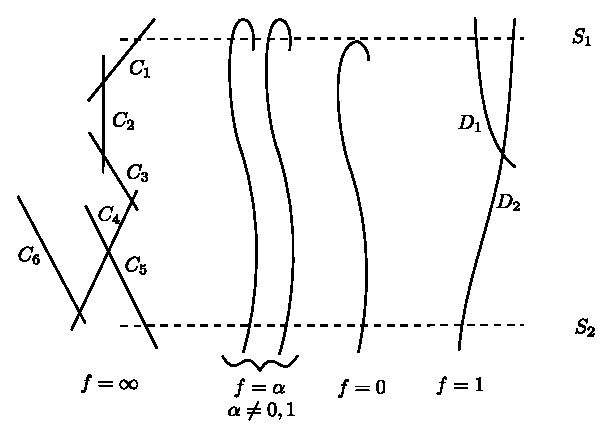
\includegraphics{figures/chap2-fig2.eps}
\end{figure}

\begin{proposition}\label{chap2-prop6}
For each of the 12 special values \eqref{chap2-eq19} the
equations \eqref{chap2-eq18} schematically define a pentagon. For
$\lambda=0$, $\infty$ the vertices are the coordinate points for
$\lambda=-\dfrac{1}{2}\epsilon^{-1}(1\pm \sqrt{5})$ the vertices are
the points $e_{kl}$, $k=0,\ldots,4$, from \ref{chap2-sec2.3}. 
\end{proposition}

In one case, say $\lambda=0$, this can be checked by hand. The other
11 cases are equivalent under the operation of $SL(2,\mathbb{Z}_{5})$:
Recall $\mu$, $\nu$, $\delta\in SL(2,\mathbb{Z}_{5})$
from \ref{chap2-sec3.1}. $\rho(\mu)$ changes $v_{i}$ to $-v_{2i}$ and
$Q_{k}(\lambda)$ into $Q_{k}(-1/\lambda)$. This transforms
$0\leftrightarrow \infty$, 
$-\dfrac{1}{2}\epsilon^{-l}(1+\sqrt{5})\leftrightarrow
-\dfrac{1}{2}\epsilon^{-l}(1-\sqrt{5})\cdot \rho(v)$ changes $v_{i}$
to $\epsilon^{-i^{2}}v_{i}$ and $Q_{k}(\lambda)$\pageoriginale into
$\epsilon^{-2k^{2}}Q_{k}(\lambda \epsilon^{3})$.

Repeated application permutes cyclically the values
$-\dfrac{1}{2}\epsilon^{-l}(1\pm \sqrt{5})$ with the same sign.

$\rho(\delta)$ transforms $e_{k}$ into a multiple of $e_{k,0}$. This
transforms the values $0$, $\infty$ into
$-\dfrac{1}{2}\epsilon^{-l}(1\pm \sqrt{5})$.\hfill$\Box$

In face the 6 five-tuplets $\{e_{k}\}$,
$\{e_{kl},k=0,\ldots,4\}l=0,\ldots,4$ are the fixed points of the 6
cyclic subgroups in $\mathbb{Z}_{5}\times \mathbb{Z}_{5}$ of order 5
operating on $\mathbb{P}_{4}$. They are permuted transitively by
$SL(2,\mathbb{Z}_{5})$. 

\subsection{The surfaces \texorpdfstring{$S_{25}$}{S25}}\label{chap2-sec3.4}

For the parameters $\lambda$ different from the 12 special values we
know that the curves $E_{\lambda}$ are smooth. Among them appear all
$H_{5}$-equivariantly embedded elliptic curves. Strictly speaking,
this does not yet imply that all the smooth $E_{\lambda}$ are such
elliptic curves. To see this, we put all the curves $E_{\lambda:\mu}$
in a flat family:

Define the surface
\begin{align*}
S_{25} &=\{(v;\lambda,\mu)\in\mathbb{P}_{4}\times \mathbb{P}_{1}:\\
&\qquad (\lambda f^{+}(v)+\mu f^{-}(v))\wedge (\lambda f^{+}(v)+\mu
f^{-}(v))=0\} 
\end{align*}
The projection onto the second factor induces a map
$S_{25}\to \mathbb{P}_{1}$. Its fibre over $(\lambda:\mu)$ projected
into $\mathbb{P}_{4}$ is just the curve $E_{\lambda:\mu}$. 

\begin{lemma}\label{chap2-lem4}
$S_{25}$\pageoriginale is a smooth surface.
\end{lemma}

\begin{proof}
We consider the differential map
{\fontsize{10pt}{12pt}\selectfont
\begin{align*}
& V\times |\mathbb{C}^{2}\to \Lambda^{4}V\\
& dv, d\lambda,d\mu\to (\lambda f^{+}(v)+\mu f^{-}(v))\wedge (\lambda
f^{+}(dv)+uf^{-}(dv)+d\lambda f^{+}(v)+d\mu f^{-}(v))
\end{align*}}
and show that its rank equals 3 for all $(\nu,\lambda,\mu)\in
S_{25}$. The map
$$
dv\to (\lambda f^{+}(v)+\mu f^{-}(v)\wedge (\lambda f^{+}(dv)+\mu f^{-}(dv))
$$
has rank 3 for all $v$ belonging to a smooth curve $E_{\lambda:\mu}$
(proposition \ref{chap2-prop3}) and for all smooth $v$ on one of the
12 singular curves $E_{\lambda:\mu}$ (proposition 6 above). This
proves the assertion for these $v$. If $v$ is one of the points
$e_{k}$, $e_{kl}$, using the symmetries we may assume $v=e_{0}$,
$\lambda=1$, $\mu=0$. The differential then is
\begin{align*}
& e_{2}\wedge e_{3}\wedge (\sum dv_{i}e_{i+2}\wedge e_{i+3}+d\lambda
e_{2}\wedge e_{3}+d\mu e_{1}\wedge e_{4})=\\
&=d\mu \widehat{e}_{0}+dv_{2}e_{1}+dv_{3}\widehat{e}_{4}
\end{align*}
and obviously has rank 3.
\end{proof}

\begin{theorem}\label{chap2-thm1}
The subscheme given by equations \eqref{chap2-eq18} is a smooth
quintic elliptic normal curve $E_{\lambda}$ embedded
$H_{5}$-equivariantly in $\mathbb{P}_{4}$ is $\lambda$ is not one of the
12 special values \eqref{chap2-eq19} a pentagon with vertices $e_{k}$,
$k=0,\ldots,4,(\lambda=0,\infty)$ or $e_{kl}$,
$k=0,\ldots,4(\lambda=-\dfrac{1}{2}\epsilon^{-l}(1\pm \sqrt{5}))$. 
\end{theorem}

\begin{proof}
For\pageoriginale $\lambda$ not one of the 12 special values we know
that $E_{\lambda}$ is smooth, isomorphic with a smooth fibre of
$S_{25}\to \mathbb{P}_{1}$. All elliptic curves appear as such fibres,
so all smooth fibres, hence all smooth $E_{\lambda}$ too are
(connected) elliptic curves. The equations \eqref{chap2-eq18} are
$H_{5}$-invariant. This implies that each smooth $E_{\lambda}$ is an
$H_{5}$-invariant elliptic quintic.
\end{proof}

\subsection{Cubic equations}\label{chap2-sec3.5}

The set $E_{\lambda:\mu}$ is described not only by the quadratic
equations \eqref{chap2-eq18} alias \eqref{chap2-eq15} but also
(cf. prop.~\ref{chap2-prop2}) by the five cubic equations equivalent
to $\lambda v^{+}-\mu v^{-}=0$
\setcounter{equation}{19}
\begin{equation}
\lambda
(v_{k+2}v^{2}_{k+4}-v^{2}_{k+3})-\mu(v_{k+1}v^{2}_{k+2}-v^{2}_{k+3}v_{k+4})=0\label{chap2-eq20} 
\end{equation}
At the 30 points $e_{k}$, $e_{kl}$ both $v^{+}$ and $v^{-}$ vanish, so
these points have to be excluded.

\begin{proposition}\label{chap2-prop7}
Away from the 30 points $e_{k}$, $e_{kl}$ the cubic
equations \eqref{chap2-eq20} define the scheme $E_{\lambda:\mu}$. 
\end{proposition}

\begin{proof}
At some $v\in E_{\lambda:\mu}$, $v\neq e_{k}$, $e_{kl}$, we compute
the rank of the differential
$$
d(\lambda v^{+}-\mu v^{-}):V\to V.
$$
For $v=\sum v_{i}e_{i}$, $dv=\sum dv_{i}e_{i}\in V$, we abbreviate
\begin{align*}
h^{+}(v,dv) &= \sfrac{1}{2}(f^{+}(v)\wedge f^{+}(dv))^{*}\\
&= \sfrac{1}{2}\sum (v_{i+4}dv_{i+4}+dv_{i+1}v_{i+4})\widehat{e}_{i}\\
h^{-}(v,dv) &=\sfrac{1}{2}(f^{-}(v)\wedge f^{-}(dv))^{*}\\
&= -\sfrac{1}{2}\sum (v_{i+2}dv_{i+3}dv_{i+2}v_{i+3})\widehat{e}_{i}\\
h^{0}(v,dv) &= (f^{+}(v)\wedge f^{-}(dv))^{*}=\sum v_{i}dv_{i}\widehat{e}_{i}
\end{align*}\pageoriginale
Differentiating $-v^{\pm}=\langle h^{0}(v), f^{\pm}(v)\rangle$ and
using \eqref{chap2-eq6}, we find
\begin{align*}
-dv^{\pm} &= \langle 2h^{0}(v,dv),f^{\pm}(v)\rangle +\langle h^{0}(v),
 f^{\pm}(dv)\rangle\\
&= \langle h^{0}(v,dv),f^{\pm}(v)\rangle -2\langle
 h^{\pm}(v,dv),f^{\mp}(v)\rangle\\
-d(\lambda v^{+}-\mu v^{-}) &= \langle \lambda h^{0}(v,dv)+2\mu
 h^{-}(v,dv),f^{+}(v)\rangle\\
&\quad -\langle \mu h^{\circ}(v,dv)+2\lambda
 h^{+}(v,dv),f^{-}(v)\rangle\\
&= \langle ((\lambda f^{+}(v)+\mu f^{-}(v))\wedge
 f^{-}(dv)^{*},f^{+}(v)\rangle\\
&\quad -\langle ((\lambda f^{+}(v)+\mu f^{-}(v))\wedge
 f^{+}(dv))^{*},f^{-}(v)\rangle 
\end{align*}
If $dv$ belongs to the kernel of the differential at $v$, then from
\begin{equation*}
\langle ((\lambda f^{+}(v)+\mu f^{-}(v))\wedge
f^{\pm}(dv))^{*}, \lambda f^{+}(v)+\mu f^{-}(v)\rangle =0\tag{6}
\end{equation*}
we deduce
$$
\langle ((\lambda f^{+}(v)+\mu f^{-}(v))\wedge (\lambda f^{+}(dv)+\mu
f^{-}(dv)))^{*}, f^{\pm}(v)\rangle =0 
$$
From\pageoriginale (9) we know $\langle
h^{+}(v),f^{+}(v)\rangle =\langle h^{-}(v), f^{-}(v)\rangle=0$. The
space of forms $h\in V^{*}$ with $\langle h, f^{+}(v)\rangle=0$ is
one-dimensional unless $f^{+}(v)$ is a simple bivector and similarly
for $f^{-}(v)$.

Applying some transformation from $SL(2,\mathbb{Z}_{5})$, we may
assume that this is not the case. Since, by assumption, we are away
from the 30 points $e_{k}$, $e_{kl}$, from
proposition \ref{chap2-prop2} (iv) we conclude $h^{+}(v)\wedge
h^{-}(v)\neq 0$. Then necessarily
$$
(\lambda f^{+}(v)+\mu f^{-}(v))\wedge (\lambda f^{+}(dv)+\mu
f^{-}(dv))=0. 
$$
So the kernel of $d(\lambda v^{+}-\mu v^{-})$ coincides with the
kernel of $d((\lambda f^{+}(v)+\mu f^{-}(v))\wedge (\lambda
f^{+}(v)+\mu f^{-}(v))$. The assertion follows from
proposition \ref{chap2-prop3} and \ref{chap2-prop6}.
\end{proof}

\section{Shioda's elliptic modular surface \texorpdfstring{$S(5)$}{S5}}\label{chap2-sec4}

\subsection{The universal elliptic curve with
level-\texorpdfstring{$n$}{n}-structure}\label{chap2-sec4.1} 

Let $\mathscr{H}$ denote the {\em upper half-plane}
$\{z\in \mathbb{C}:\text{Im}~z>0\}$. Each $z\in \mathscr{H}$ defines an
elliptic curve $E_{z}=\mathbb{C}/\mathbb{Z}+\mathbb{Z}z$ and in
$H_{1}(E_{z},\mathbb{Z})$ a distinguished basis $s_{z}$, $t_{z}$,
namely, the images of $1$, $z$ under the canonical isomorphism
$\mathbb{Z}+\mathbb{Z}_{z}\to H_{1}(E_{z},\mathbb{Z})$. Clearly, the
intersection number is $s_{z}\cdot t_{z}=1$. The complex numbers\pageoriginale
$\dfrac{1}{n}$, $\dfrac{z}{n}$ have image points $\sigma_{z}$,
$\tau_{z}\in E^{(n)}_{z}$ forming a symplectic basis for $E^{(n)}_{z}$.

\begin{lemma}\label{chap2-lem5}
Each elliptic curve $E$ with level-$n$-structure defined by a
symplectic basis $\alpha$, $\beta\in E^{(n)}$ is isomorphic to
$(E_{z};\sigma_{z},\tau_{z})$ for some $z\in \mathscr{H}$.
\end{lemma}

\begin{proof}
Write $E=\mathbb{C}/\Omega$ and let $a$, $b$, $\in \mathbb{C}$ be
inverse images of $\alpha$, $\beta$ such that $na$,
$nb\in \Omega=H_{1}(E,\mathbb{Z})$ have intersection number $(na)\cdot
(nb)=1$. This implies $z:=nb/na\in \mathscr{H}$. Under multiplication
$\mathbb{C}\to \mathbb{C}$, $\zeta\to \zeta/na$, the lattice $\Omega$
is mapped onto $\mathbb{Z}+\mathbb{Z}z$ with $na\to 1$, $nb\to
z$. This induces an isomorphism $E\to E_{z}$ with
$\alpha\to \sigma_{z}$, $\beta\to \tau_{z}$.
\end{proof}

On $\mathscr{H}$ operates the group $\Gamma=SL(2,\mathbb{Z})$ by
$$
\gamma z=\dfrac{az+b}{cz+d}\quad\text{for}\quad \gamma=
\begin{pmatrix}
a & b\\
c & d
\end{pmatrix}
\in \Gamma
$$
The elliptic curves $E_{z}$ and $E_{z}$ are isomorphic if and only if
$z'=\gamma z$ for some $\gamma\in \Gamma$. Explicitly, the isomorphism
$E_{z}\to E_{\gamma z}$ is given as follows: multiplication $\zeta\to
(cz+d)^{-1}\zeta$ induces an isomorphism
$$
E_{z}=\mathbb{C}/\mathbb{Z}(cz+d)+\mathbb{Z}(az+b)\to \mathbb{C}/\mathbb{Z}+\mathbb{Z}\dfrac{az+b}{cz+d}=E_{\gamma
z}. 
$$
Under\pageoriginale this isomorphism, the basis
\begin{align*}
& 1=a(cz+d)-c(az+b)\\
& z=-b(cz+d)+d(az+b)
\end{align*}
of $H_{1}(E_{z},\mathbb{Z})$ goes to the basis $a-c\gamma z$,
$-b+d\gamma z$ of $H_{1}(E_{\gamma z},\mathbb{Z})$. The
level-$n$-structure given on $E_{z}$ by $\sigma_{z}$, $\tau_{z}$ goes
on $E_{\gamma z}$ to the one determined by $a\sigma_{\gamma z}$,
$-c\tau_{\gamma z}$, $-b\sigma_{\gamma z}+d\tau_{\gamma z}$.

Denote by $\Gamma(n)\subset \Gamma$ the {\em congruence subgroup}
$$
\{\gamma\in \Gamma:\gamma\equiv 1\text{~ mod~ } n\}.
$$

\begin{lemma}\label{chap2-lem6}
Two curves with level-$n$-structure, 
$$
(E_{z},\sigma_{z},\tau_{z})\quad\text{and}\quad
(E_{z'},\sigma_{z'},\tau_{z})
$$ 
are isomorphic if and only if
$z'=\gamma z$ with $\gamma\in \Gamma(n)$. 
\end{lemma}

\begin{proof}
If $z'=\gamma z$, $\gamma\in \Gamma(n)$, then, by the above, there is
an isomorphism $E_{z}\to E_{z'}$, mapping $\sigma_{z}\to \sigma_{z'}$
and $\tau_{z}\to \tau_{z'}$.

Assume, conversely, that $(E_{z},\sigma_{z},\tau_{z})$ and
$(E_{z'},\sigma_{z'},\tau_{z'})$ are isomorphic. Then there is some
$\gamma\in \Gamma$ with $z'=\gamma z$ and $a\sigma_{z'}-c\tau_{z'}$,
$-b\sigma_{z'}+d\tau_{z'}$ differs from the symplectic basis
$\sigma_{z'}$, $\tau_{z'}\in E^{(n)}_{z'}$ by an automorphism $r$ of
$E_{z'}$. Then there is some $\rho=\left(\begin{smallmatrix} p & q\\ s
& t\end{smallmatrix}\right)\in \Gamma$ such that $\rho z'=z'$ and 
\begin{align*}
& a\sigma_{z'}-c\tau_{z'}=r_{*}\sigma_{z'}=p\sigma_{z'}-s\tau_{z'},\\
& -b\sigma_{z'}+d\tau_{z'}=r_{*}\tau_{z'}=-q\sigma_{z'}+t\tau_{z'}.
\end{align*}\pageoriginale
Then $\rho^{-1}\gamma\in \Gamma$ maps $z\to z'$,
$\sigma_{z}\to \sigma_{z'}$, $\tau_{z}\to \tau_{z'}$ and from this, it
follows in particular that $\rho^{-1}\gamma\in \Gamma(n)$. 
\end{proof}

The last lemma means that there is a bijective correspondence between
points of $X'(n):=\mathscr{H}/\Gamma(n)$ and isomorphism classes of
elliptic curves with level-$n$-structure. Assume $n\geq 3$, from now
on. Then the action of $\Gamma(n)$ on $\mathscr{H}$ has no fixed
points.

We denote by $N$ the semi-direct product $\Gamma\times
(\mathbb{Z}\times \mathbb{Z})$, i.e. the set $\Gamma\times
(\mathbb{Z}\times \mathbb{Z})$ with the group law
$$
(\gamma,(m_{1},m_{2}))\cdot
(\gamma',(m'_{1},m'_{2}))=(\gamma\gamma',(m_{1},m_{2})\cdot \gamma'+(m_{1},m'_{2})). 
$$
This group $N$ acts on $\mathscr{H}\times \mathbb{C}$ by
\begin{equation}
(\gamma,(m_{1},m_{2})):(z,\zeta)\to (\gamma
z,(\zeta+m_{1}z+m_{2})(cz+d)^{-1}). \label{chap2-eq21}
\end{equation}
Since $n\geq 3$, the induced action of $\Gamma(n)\times
(\mathbb{Z}\times \mathbb{Z})$ has no fixed points and
$$
S'(n)=\mathscr{H}\times \mathbb{C}/\Gamma(n)\times
(\mathbb{Z}\times \mathbb{Z}) 
$$
is a smooth surface. The
projection. $\mathscr{H}\times \mathbb{C}\to \mathscr{H}$ induces a
map $\varphi:S'(n)\to X'(n)$. The fibre over $(z\mod \Gamma(n))\in
X'(n)$ is isomorphic with the curve $E_{z}$. The set
$\{(z,0)\in \mathscr{H}\times \mathbb{C}:z\in \mathscr{H}\}$ is
invariant under the group action. Its image in $S'(n)$ is a
section\pageoriginale $L_{0,0}$ for $\varphi$ meeting each fibre in
its origin. Similarly, the sets
$\{(z,\dfrac{1}{n}):z\in \mathscr{Z}\}$,
$\{(z,\dfrac{z}{n}):z\in \mathscr{H}\}$ define sections $L_{1,0}$,
$L_{0,1}$ for $\varphi$ meeting each fibre in the image of
$\sigma_{z}$, $\tau_{z}$. So the two sections $L_{1,0}$, $L_{0,1}$
provide each fibre of $\varphi$ with a
level-$n$-structure. Lemmas \ref{chap2-lem5} and \ref{chap2-lem6} mean
that each elliptic curve with level-$n$-structure is isomorphic to
exactly one fibre. In this sense, $\varphi:S'(n)\to X'(n)$ with zero
section $L_{0,0}$ and the two sections $L_{1,0}$, $L_{0,1}$ is the
universal elliptic curve with level-$n$-structure. 

\subsection{Shioda's elliptic surface \texorpdfstring{$S(n)$}{Sn} for \texorpdfstring{$n\geq 3$}{n3}}\label{chap2-sec4.2} 

By adding cusps, the curve $X'(n)$ is completed. The result is the
{\em modular curve} $X(n)$. Shioda \cite[p.38]{chap2-key11} has shown
how to complete the surface $S'(n)$ by adding over each cusp a
singular fibre of type $I_{n}$, i.e., an $n$-gon of projective
lines. The result is the smooth compact {\em modular surface} $S(n)$,
fibred over the modular curve $X(n)$ by $\varphi:S(n)\to X(n)$.

The two sections $L_{1,0}$, $L_{0,1}$ generate a group of $n$-torsion
sections for $\varphi:S'(n)\to X'(n)$. This group is isomorphic to
$\mathbb{Z}_{n}\times \mathbb{Z}_{n}$. Shioda shows that those
sections extend over all of $X(n)$, and that the $n^{2}$ sections
obtained in this way are the only sections for $\varphi:S(n)\to
X(n)$ \cite[theorem 5.5]{chap2-key11}. Of course, over $X'(n)$, the
$n^{2}$ sections are always disjoint. This is also true over the
cusps: Each line in one of the $n$-gons is met by $n$ sections in $n$
different points.

By\pageoriginale Kodaira's theory, cf. \cite[V theorem
11.1(b)]{chap2-key2}, the surface $S(n)$ is uniquely determined by
$S'(n)$ and one extended section. In particular, each automorphism of
$S'(n)$, mapping the $n$-torsion sections into themselves, extends
uniquely to an automorphism of $S(n)$. We therefore have, acting on
$S(n)$,
\begin{itemize}
\item[--] the group $\mathbb{Z}_{n}\times \mathbb{Z}_{n}$ of
$n$-torsion sections. Denote by $L_{k,l}$ the section corresponding to
$(k.l)\in \mathbb{Z}_{n}\times\mathbb{Z}_{n}$

\item[--] the quotient $SL(2,\mathbb{Z}_{n})=\Gamma/\Gamma(n)$. Its
action is induced by the action \eqref{chap2-eq21} of $N$.
\end{itemize}

Now $\gamma=\left(\begin{smallmatrix} a & b\\ c &
d\end{smallmatrix}\right)\in T$ maps
\begin{align*}
& L_{1,0}\to L_{a,-c}\qquad L_{0,1}\to L_{-b,d}\\
& \mathbb{Z}_{n}\times \mathbb{Z}_{n}\ni \binom{k}{l}
\to\begin{pmatrix}
a & -b\\
-c & d
\end{pmatrix}
\binom{k}{l}
\end{align*}
where
$$
\begin{pmatrix}
a & -b\\
-c & d
\end{pmatrix}
=
\left\{\left[
\begin{pmatrix}
0 & 1\\
1 & 0
\end{pmatrix}
\gamma
\begin{pmatrix}
0 & 1\\
1 & 0
\end{pmatrix}
\right]^{t}\right\}^{-1}=:\gamma'
$$
So up to the automorphism $\gamma\to \gamma'$ of
$SL(2,\mathbb{Z}_{n})$ this is the action of $SL(2,\mathbb{Z}_{n})$ on
$\mathbb{Z}_{n}\times \mathbb{Z}_{n}$ from \ref{chap2-sec3.1}. The
semi-direct product\pageoriginale $SL(2,\mathbb{Z}_{n})\times
(\mathbb{Z}_{n}\times \mathbb{Z}_{n})$ with respect to this action
operates on $S(n)$. Shioda \cite{chap2-key11} remarks that this is the
full automorphism group of $S(n)$. Notice that it is the central
quotient $N_{n}/\mathbb{Z}_{n}$ with $N_{n}$ from \ref{chap2-sec3.1}.

\subsection{Divisors on the surface \texorpdfstring{$S(5)$}{S5}}\label{chap2-sec4.3}

The modular curve $X(5)$ is rational, obtained from $X'(5)$ by adding
12 cusps \cite[p.23]{chap2-key10}. The surface $S(5)$ therefore
contains 12 fibres of type $I_{5}$ (pentagons). Summing over the 12
pentagons, we obtain the Euler number of $S(5)$
$$
e=60.
$$
This implies
\begin{alignat*}{2}
& X(\mathscr{O}_{S(5)})=5 &\qquad& \text{(Noether's formula)}\\
& K_{S(5)}=\mathscr{O}_{S(5)}(3F), &\qquad& \text{(Kodaira's formula)}
\end{alignat*}
where $F$ is the class of a fibre,
$$
P_{g}=4, q=b_{1}=0, b_{2}=58, h^{1,1}=50.
$$

\begin{lemma}\label{chap2-lem7}
The Picard group $Pic\ S(5)$ contains no torsion.
\end{lemma}

\begin{proof}
\cite{chap2-key13} Corollary 1.

On $S(5)$, we have the following divisor classes:

$F$ the class of a fibre,

$L_{k,l}~~k,l=0,\ldots,4$, the 25 sections,

$F_{1},\ldots,F_{12}$ the twelve singular fibres.

For $i=1,\ldots,12$, we let $F_{i,0}\subset F_{i}$ be the component
meeting $L_{0,0}$\pageoriginale and label the other components
$F_{i,k}$, $k=1,2,3,4$, in such a way that $F_{i,k}\cdot
F_{i,k+1}=1(k=0,\ldots,4\text{~ mod~ }5)$. This determines the
notation uniquely up to a change of orientation in the pentagons. We
have the following intersection numbers
\begin{align*}
& F^{2}=0, F\cdot L_{k,l}=1,\quad F\cdot F_{i,k}=0\\
& L^{2}_{k,l}=-5,\quad F^{2}_{i,k}=-2
\end{align*}
and each $F_{i,k}$ meets exactly five $L_{k,l}$.
\end{proof}

\begin{lemma}\label{chap2-lem8}
The 50 classes $L_{0,0}$, $F$, and $F_{i,k}$, $i=1,\ldots,12$;
$k=1,2,3,4$, form a basis of $\Pic (S(5))\otimes \mathbb{Q}$.
\end{lemma}

\begin{proof}
Since $h^{1,1}(S(5))=50$, it will be sufficient to compute the
intersection matrix of these divisor classes. One finds
$$
\begin{pmatrix}
-5 & 1 & & & \\
1 & 0 & &&\\
  &   & A_{4} & &\\
      &&& \ddots\\
 & & & & A_{4}
\end{pmatrix}
\quad\text{where}\quad A_{4}=
\begin{pmatrix}
-2 & 1 & &\\
1 & -2 & 1 & \\
  & 1 & -2 & 1\\
  &   & 1 & -2
\end{pmatrix}
$$
There are 12 blocks $A_{4}$, each with determinant 5. So the
intersection matrix has determinant $-5^{12}\neq 0$.
\end{proof}

Next, we define the divisor class
\begin{equation}
I:5L_{0,0}+24F-\sum^{12}_{i=1}\left(2F_{i,1}+3F_{i,2}+3F_{i,3}+2F_{i,4}\right)\label{chap2-eq22} 
\end{equation}
This\pageoriginale definition, looking somewhat artificial, is
motivated by the following fact.

\begin{lemma}[Inoue, Livne]\label{chap2-lem9}
In $\Pic(S(5))$ one has
$$
5I=\sum_{k,l}L_{k,l}
$$
\end{lemma}

\begin{proof}
By lemma \ref{chap2-lem7}, it suffices to prove that both divisors are
numerically equivalent. By lemma \ref{chap2-lem8}, this follows from
the equations
\begin{align*}
& (L:=\sum L_{k,l})\\
&\qquad L\cdot L_{0,0}=-5=5I\cdot L_{0,0}\\
&\qquad L\cdot F=25=5I\cdot F\\
&\qquad L\cdot F_{i,1}=L\cdot F_{i,4}=5=5I\cdot F_{i,1}=5I\cdot
F_{i,4}\\
&\qquad L\cdot F_{i,2}=L\cdot F_{i,3}=5=5I\cdot F_{i,2}=5I\cdot
F_{i,3}.  
\end{align*}
\end{proof}

The divisor classes $F$ and $I$ are invariant under the action of
$$
\Aut (S(5))=SL(2,\mathbb{Z}_{5})\times
(\mathbb{Z}_{5}\times \mathbb{Z}_{5}).
$$ 

\begin{lemma}\label{chap2-lem10}
Any class $D\in \Pic(S(5))$ invariant under the group
$\mathbb{Z}_{5}\times \mathbb{Z}_{5}$ of translations by 5-torsion
sections is of the form $D=pI+qF$, $p$, $q\in \mathbb{Z}$. 
\end{lemma}

\begin{proof}
By\pageoriginale  lemma \ref{chap2-lem8}, there are $a$, $b$,
$c_{ik}\in \mathbb{Q}$ such that 
$$
D=aL_{0,0}+bF+\sum^{12}_{i=1}\sum^{4}_{k=1}c_{ik}F_{ik}
$$
If $D$ is invariant, then
\begin{align*}
D
&= \frac{1}{25}\sum_{\alpha\in \mathbb{Z}_{5}\times \mathbb{Z}_{5}}\alpha\ast
D\\
&= \dfrac{a}{25}\sum L_{k,l}+bF+5\sum^{12}_{i=1}\sum_{k=1}c_{ik}F\\
&= \frac{a}{5}I+(b+5\sum c_{ik})F.
\end{align*}
This shows $D=pI+qF$ with $p$, $q\in \mathbb{Q}$. But
$$
p=D\cdot F_{1,0}\in \mathbb{Z},\quad q-p=D\cdot L_{0,0}\in \mathbb{Z}
$$
\end{proof}

The action of the translation group
$\mathbb{Z}_{5}\times \mathbb{Z}_{5}$ lifts trivially to an action on
$\mathscr{O}_{S(5)}(F)$. To $\mathscr{O}_{S(5)}(I)$, it lifts as an
action of the Heisenberg group: Let $\sigma$,
$\tau\in \mathbb{Z}_{5}\times \mathbb{Z}_{5}$ be the distinguished
generators (cf.~\ref{chap2-sec4.1}) with $\sigma(L_{0,0})=L_{1,0}$,
$\tau(L_{0,0})=L_{0,1}$. Denote by $O_{E}$ the point $L_{0,0}\cap E$
for any fibre $E$. The explicit formula \eqref{chap2-eq22} shows
$\mathscr{O}_{E}(I)=\mathscr{O}_{E}(50_{E})$ for any smooth fibre
$E$. We therefore may lift $\sigma$, $\tau$ to $\mathscr{O}_{S(5)}(I)$
such that over one fixed smooth fibre $E$ they act as
in \ref{chap2-sec3.2}. This implies
$\sigma\tau\sigma^{-1}\tau^{-1}=\epsilon$. id on all of
$\mathscr{O}_{S(5)}(I)$, i.e. the Heisenberg group $H_{5}$ acts on
$S(5)$ covering the translation group on
$S(5)$. By \ref{chap2-sec3.2}, the action of $H_{5}$ on
$\mathscr{O}_{E}(50_{E})$ is uniquely determined by the symplectic
basi $\sigma$,\pageoriginale $\tau\in E^{(5)}$ up to an inner
automorphism of $H_{5}$. So the action of $H_{5}$ on all the smooth
fibres $E$ is isomorphic to the one described in \ref{chap2-sec3.2}.

By tensor products, we define an action of $H_{5}$ on all line bundles
$\mathscr{O}_{S(5)}(pI+qF)$, $p$, $q\in Z$.

\subsection{The linear system \texorpdfstring{$|I+2F|$}{I2F} on \texorpdfstring{$S=S(5)$}{SS5}.}\label{chap2-sec4.4}


Here we want to describe the map defined by the linear system $|I+2F|$
on $S$.

\begin{proposition}\label{chap2-prop8}
Let $D=pI+qF$ be a divisor on $S$. Then
\begin{itemize}
\item[\rm(i)] $D$ is ample if and only if $q>p>0$.

\item[\rm(ii)] $h^{1}(\mathscr{O}_{S}(D))$ vanishes if $p>0$, $q>p+3$.

\item[\rm(iii)] $h^{2}(\mathscr{O}_{S}(D))$ vanishes if $p>0$.
\end{itemize}
\end{proposition}

\begin{proof}
\begin{itemize}
\item[(i)] If $D$ is ample, then $5p=D\cdot F>0$ and $q-p=D\cdot
L_{0,0}>0$. To prove the converse, we use the Nakai-Moishezon
criterion: If $q>p>0$, then $D^{2}=5p(2q-p)>0$. If $C\subset S(5)$ is
an irreducible curve, then $C\cdot F>0$ and $C\cdot I\geq 0$, hence
$C\cdot D>0$, unless one of the following holds:
\begin{itemize}
\item[(a)] $C$ is a section. Then $C\cdot D=q-p>0$

\item[(b)] $C$ is a smooth fibre. Then $C\cdot D=5p>0$.

\item[(c)] $C$\pageoriginale is a component of a singular fibre. Then
$C\cdot D=p>0$.
\end{itemize}
\item[(ii)] follows from Kodaira's vanishing theorem and (i), because
$K_{S}=\mathscr{O}_{S}(3F)$. 

\item[(iii)] We have
$h^{2}(\mathscr{O}_{S}(D))=h^{\circ}(\mathscr{O}_{S}(K-D))$ and
$K-D=-pI+(3-q)F$ cannot be effective if $p>0$.
\end{itemize}
\end{proof}

\begin{lemma}\label{chap2-lem11}
For $D=I+qF$ we have the following table:
$$
\begin{array}{r@{\;}c@{\qquad}c@{\qquad}c@{\qquad}c}
& q & \chi(D)=5q-5 & h^{\circ}(D) & h^{1}(D)\\[5pt]
& 0 & -5 & 0 & 5\\[5pt]
&1 & 0 & 0 & 0\\
\geq & 2 & 5q-5 & 5q-5 & 0
\end{array}
$$
\end{lemma}

\begin{proof}
Applying Riemann-Roch to $D$, we find
\begin{align*}
\chi(D) & = \frac{1}{2}D\cdot (D-K)+\chi(\mathscr{O}_{S})\\[5pt]
&= \frac{1}{2}(I+qF)\cdot (I+(q-3)F)+5\\[5pt]
&= 5q-5
\end{align*}
For $q\geq 1$, we show $h^{1}(D)=0$ by descending induction on $q$. If
$q\geq 5$, the assertion follows from
proposition \ref{chap2-prop8}. Assume $q\geq 1$ and consider, for a
smooth fibre $E$, the exact sequence 
$$
0\to \mathscr{O}_{S}(I+qF)\to \mathscr{O}_{S}(I+(q+1)F)\to \mathscr{O}_{E}(5O_{E})\to 0
$$\pageoriginale
By induction, $h^{1}(\mathscr{O}_{S}(I+(q+1)F))=0$ and we obtain a
$H_{5}$-equivariant exact sequence
$$
H^{\circ}(\mathscr{O}_{S}(I+(q+1)F))\xrightarrow{\rm restr.}
H^{\circ}(\mathscr{O}_{E}(5O_{E}))\to H^{1}(\mathscr{O}_{S}(I+qF))\to 0.
$$
In view of $h^{1}(\mathscr{O}_{S}(I+(q+1)F))=0$, we have
$h^{\circ}(O_{S}(I+(q+1)F))\neq 0$. So the restriction map cannot
vanish for all $E$. But the $H_{5}$-space
$H^{\circ}(\mathscr{O}_{E}(5O_{E}))$ is irreducible, so restr is
surjective for general $E$ and the assertion follows for $q\geq
1$. But, if $\mathscr{O}_{S}(I+F)$ has no sections, the same is true
for $\mathscr{O}_{S}(I)$.
\end{proof}

\begin{lemma}\label{chap2-lem12}
The linear system $|I+2F|$ has no base points on $S$.
\end{lemma}

\begin{proof}
Lemma \ref{chap2-lem11} implies that restriction
$$
H^{\circ}(\mathscr{O}_{S}(I+2F))\to H^{\circ}(\mathscr{O}_{E}(I))
$$
is bijective for all fibres $E$. If $E$ is smooth, then
$\mathscr{O}_{E}(I)=\mathscr{O}_{E}(5O_{E})$ and $E$ cannot contain
any base points. So assume that $E=\bigcup\limits^{4}_{k=0}F_{i,k}$ is
a pentagon. The restriction $\mathscr{O}_{F_{i,k}}(I)$ has degree 1 on
each component $F_{i,k}$. If a smooth point $p\in E$ would be a base
point, then by $\mathbb{Z}_{5}\times \mathbb{Z}_{5}$ symmetry there
would be 25 such points on $E$ and all sections in
$\mathscr{O}_{E}(I)$ would vanish, a contradiction. If a singular
point $p\in E$ would be a base point, then\pageoriginale by
$\mathbb{Z}_{5}\times \mathbb{Z}_{5}$-symmetry each component
$F_{i,k}$ would contain two base points, which leads to the same
contradiction. 
\end{proof}

\subsection{The surface \texorpdfstring{$S_{15}$}{S15}.}\label{chap2-sec4.5}

In view of lemma \ref{chap2-lem12} above, the linear system $|I+2F|$
defines a map $S(5)\to \mathbb{P}_{4}$. We normalize it by identifying
$H^{\circ}(\mathscr{O}_{S}(I+2F))=V^{*}$ equivariantly with respect to
the action of the Heisenberg group $H_{5}$. 

\begin{proposition}\label{chap2-prop9}
The linear system $|I+2F|$ maps the modular surface onto a surface
$S_{15}\subset \mathbb{P}_{4}$ of degree $15$. The map is injective
except for the $60$ double points of the $12$ singular fibres. The
fibres are paired and the $5$ double points on both fibres in one pair
have the same $5$ image points.
\end{proposition}

\begin{proof}
The map $S(5)\to \mathbb{P}_{4}$ is $H_{5}$-equivariant. The fibres on
$S(5)$ therefore go the $H_{5}$-invariant curves. The smooth fibres go
to the smooth quintics from \ref{chap2-sec3.3} Two different fibres
are not isomorphic as curves with level-5-structure
(see \ref{chap2-sec4.1}), so they have different image curves
$E_{\lambda}$. By proposition \ref{chap2-prop2}, the images are even
disjoint. So the map is injective on the open part $S'(5)\subset S(5)$
and the image must be surface $S_{15}$ of degree 
$$
(I+2F)^{2}=15.
$$
The\pageoriginale 12 singular fibres go to non-degenerate
$H_{5}$-invariant pentagons in $\mathbb{P}_{4}$. The vertices of such
a pentagon are fixed points for some cyclic subgroup
$\mathbb{Z}_{5}\subset \mathbb{Z}_{5}\times \mathbb{Z}_{5}$ hence
belong to the 30 points $e_{k}$, $e_{k,l}$. It follows that each
singular fibre is mapped isomorphically to one of the 12 singular
curves $E_{\lambda}$. Conversely, all curves $E_{\lambda}$ are images
of fibres on $S(5)$. This follows because the curves $E_{\lambda}$
sweep out the irreducible surface which is the projection of
$S_{25}\subset \mathbb{P}_{4}\times \mathbb{P}_{1}$
from \ref{chap2-sec3.4} into $\mathbb{P}_{4}$. This projection
necessarily coincides with $S_{15}$ so each $E_{\lambda}$ is contained
in the image. By proposition \ref{chap2-prop2}, all $E_{\lambda}$ are
disjoint, except for the pairs of singular ones which have the same
vertices. This proves the assertion.
\end{proof}

Next, we show that $S_{15}$ is smooth, except for the 30 double points
$e_{k}$, $e_{k,l}$, where two smooth branches of $S_{15}$ cross
transversally. This follows from

\begin{proposition}\label{chap2-prop10}
\begin{itemize}
\item[\rm(i)] The projection $S_{25}\to S_{15}$ is an immersion.

\item[\rm(ii)] The two branches of $S_{15}$ meeting in one of the $30$
points $e_{k}$, $e_{k,l}$, are transversal.
\end{itemize}
\end{proposition}

\begin{proof}
At $(v;\lambda,\mu)\in S_{25}$ the tangent space to this surface is
given by those $dv$, $d\lambda$ for which
$$
(\lambda f^{+}(v)+\mu f^{-}(v))\wedge (\lambda f^{+}(dv)+\mu
f^{-}(dv)+d\lambda f^{+}(v)+d\mu f^{-}(v))=0. 
$$
The projection has maximal rank on this tangent space unless it
contains all vectors $(0;d\lambda, d\mu)$. But this would imply
$$
2\lambda h^{+}(v)+\mu h^{\circ}(v)=\lambda h^{\circ}(v)+2\mu h^{-}(v)=0.
$$
Now,\pageoriginale recall that
$$
\lambda^{2}h^{+}(v)+\lambda \mu h^{\circ}(v)+\mu^{2}h^{-}(v)=0
$$
is the only relation between $h^{+}$, $h^{\circ}$, and $h^{-}$ unless
$v=e_{k}$ or $e_{k,l}$. So, for $v\neq e_{k}$, $e_{kl}$, we find
$\lambda \mu=0$, which eventualy leads to the contradiction
$h^{\circ}(v))=0$. 

If $v$ is one of the 30 singular points on $S_{15}$ we may assume
$v=e_{0}$, without loss of generality. The two points $(e_{0};1,0)$
and $(e_{0};0,1)$ lie on $S_{25}$ over $e_{0}$. The two tangent planes
to $S_{25}$ are 
\begin{align*}
& \mu=0:f^{+}(e_{0})(f^{+}(dv)+d\mu
f^{-}(e_{0}))=dv_{2}\widehat{e}_{1}+dv_{3}\widehat{e}_{4}+d\mu\widehat{e}_{0}=0\\
& \lambda=0:f^{-}(e_{0})(f^{-}(dv)+d\lambda
f^{+}(e_{0}))=-dv_{1}\widehat{e}_{3}-dv_{4}\widehat{e}_{2}+d\lambda \widehat{e}_{0}=0. 
\end{align*}
They project in $\mathbb{P}_{4}$ to the two planes $v_{2}=v_{3}=0$ and
$v_{1}=v_{4}=0$. They are tangent to the two branches of $S_{15}$ at
$e_{0}$ and transversal.
\end{proof}

Finally, we consider the equations defining $S_{15}$. By definition,
$S_{15}$ is the set of points $v$ where $h^{+}(v)\wedge
h^{\circ}(v)\wedge h^{-}(v)=0$. i.e.\@ the determinantal locus where
the matrix 
$$
\begin{pmatrix}
v^{2}_{0} & v^{2}_{1} & v^{2}_{2} & v^{2}_{3} & v^{2}_{4}\\[4pt]
v_{2}v_{3} & v_{3}v_{4} & v_{4}v_{0} & v_{0}v_{1} & v_{1}v_{2}\\[4pt]
v_{1}v_{4} & v_{2}v_{0} & v_{3}v_{1} & v_{4}v_{2} & v_{0}v_{3}
\end{pmatrix}
$$\pageoriginale
drops its rank. Its ten $3\times 3$ determinants, the 10 coefficients
of $v^{+}\wedge v^{-}$ are $(k=0,\ldots,4)$.
\begin{equation}
\begin{split}
&
v_{k}v_{k+2}v_{k+3}(v_{k+2}v^{2}_{k+4}-v^{2}_{k+1}v^{2}_{k+3})+v^{3}_{k}(v^{2}_{k+3}v_{k+4}-v_{k+1}v^{2}_{k+2})\\
&\hspace{1.5cm}
+v_{k+1}v_{k+4}(v^{3}_{k+1}v^{3}_{k+2}-v_{k+3}v^{3}_{k+4})\\
&
v_{k}v_{k+1}v_{k+4}(v_{k+1}v^{2}_{k+2}-v^{2}_{k+3}v_{k+4})+v^{3}_{k}(v_{k+2}v^{2}_{k+4}-v^{2}_{k+1}v_{k+3})\\
&\hspace{1.5cm} +v_{k+2}v_{k+3}(v_{k+1}v^{3}_{k+3}-v^{3}_{k+2}v_{k+4})
\end{split}\label{chap2-eq23}
\end{equation}

\begin{proposition}\label{chap2-prop11}
The ten equations \eqref{chap2-eq23} schematically define $S_{15}$.
\end{proposition}

\begin{proof}
As usual, we distinguish between two cases:
\begin{itemize}
\item[--] If $v\in S_{15}$ is a smooth point, we check that the
differential
$$
d(v^{+}\wedge v^{-}):V\to \Lambda^{2}V
$$
has rank 2. Since $v^{-}=(\lambda/\mu)v^{+}$ (if e.g.\@ $\mu\neq 0$)
we find
\begin{align*}
d(v^{+}\wedge v^{-})|_{v} &= dv^{+}|_{v}\wedge v^{-}+v^{+}\wedge
dv^{-}|_{v}\\
&= ((\lambda/\mu)v\wedge d^{+}|_{v}-dv^{-}|_{v})\wedge v^{+}.
\end{align*}
From \ref{chap2-sec3.5}, Proposition \ref{chap2-prop7}, we know that
the differential $d(\lambda v^{+}-\mu v^{-})$, $\lambda$, $\mu$ fixed,
has rank 3. This implies that our differential has rank $\geq 2$.

\item[--] If\pageoriginale $v\in S_{15}$ is a singular point, we
assume $v=e_{0}$, without loss of generality. The two branches of
$S_{15}$ at $e_{0}$ are given by functions $g_{2}$, $g_{3}$ and
$g_{1}$, $g_{4}\in \mathscr{O}_{e_{0}}$ respectively, where we may
assume that $g_{i}-v_{i}$ belongs to $m^{2}$, $m$ the ideal generated
by $v_{1}$, $v_{2}$, $v_{3}$, $v_{4}$ at $e_{0}$. Then the ideal of
$S_{15}$ is generated by $g_{1}g_{2}$, $g_{1}g_{3}$, $g_{2}g_{4}$, and
$g_{3}g_{4}$. 
\end{itemize}
\end{proof}

On the other hand, putting $v_{0}=1$ in equations \eqref{chap2-eq23}
and reducing modulo $m^{3}$ we obtain (only terms containing
$v^{4}_{0}$ ramain): $v_{1}v_{2}$, $v_{1}v_{3}$, $v_{2}v_{4}$,
$v_{3}v_{4}$. So among the 10 polynomials \eqref{chap2-eq23}, we may
pick four ones, say $h_{1},\ldots,h_{4}$ such that
$$
g_{1}g_{2}-h_{1}\equiv g_{1}g_{3}-h_{2}\equiv g_{2}g_{4}-h_{3}\equiv
g_{3}g_{4}-h_{4}\equiv 0\mod m^{3}.
$$
The polynomials $h_{1},\ldots,h_{4}$ belong to the ideal of $S_{15}$,
so we may write them
$$
h_{i}=c^{12}_{i}g_{1}g_{2}+c^{13}_{i}g_{1}g_{4}+c^{24}_{i}c_{2}g_{4}+c^{34}_{i}g_{3}g_{4},c^{kl}_{i}\in \mathscr{O}_{e_{0}}. 
$$
The congruences above imply
\begin{align*}
& c^{12}_{1}\equiv c^{13}_{2}\equiv c^{24}_{3}\equiv c^{34}_{4}\equiv
1\mod m\\[4pt]
& c^{kl}_{i}\in m\text{~~ otherwise.}
\end{align*}
The\pageoriginale $4\times 4$-matrix
$$
\begin{pmatrix}
c^{12}_{1} & c^{12}_{2} & c^{12}_{3} & c^{12}_{4}\\[4pt]
c^{13}_{1} & c^{13}_{2} & c^{13}_{3} & c^{13}_{4}\\[4pt]
c^{24}_{1} & c^{24}_{2} & c^{24}_{3} & c^{24}_{4}\\[4pt]
c^{34}_{1} & c^{34}_{2} & c^{34}_{3} & c^{34}_{4}
\end{pmatrix}
$$
therefore admits an inverse with coefficients in
$\mathscr{O}_{e_{0}}$.

We therefore may express $g_{1}g_{2}$, $g_{1}g_{3}$, $g_{2}g_{4}$,
$g_{3}g_{4}$ in the functions $h_{1},\ldots,h_{4}$. This implies that
the functions \eqref{chap2-eq23} generate the ideal of $S_{15}$ at
$e_{0}$. 

\section{Jumping lines of the Horrocks-Mumford
bundle}\label{chap2-sec5}

\subsection{Jumping lines belonging to \texorpdfstring{$v\in V$}{vV}.}\label{chap2-sec5.1}

The Horrocks-Mumford bundle $\mathscr{F}$ is stable with
$c_{1}=5$. Therefore, we have
$\mathscr{F}|L=\mathscr{O}_{\mathbb{P}_{1}}(2)\oplus \mathscr{O}_{\mathbb{P}_{1}}(3)$
for the general line $L\subset \mathbb{P}_{4}$ (Grauert-Mulich). We
define the {\em jumping order} $k(L)$ for each line
$L\subset \mathbb{P}_{4}$ by
$$
\mathscr{F}|L=\mathscr{O}_{\mathbb{P}_{1}}(2-k)\oplus \mathscr{O}_{\mathbb{P}_{1}}(3+k). 
$$
So $L$ is a {\em jumping line} (resp. {\em double, triple jumping
line}) if $k(L)\geq 1$ (resp. $k(L)\geq 2,3$). By \cite[proposition
1]{chap2-key1}, this jumping order\pageoriginale equals the dimension of the kernel
of the map
$$
V\to 2\Lambda^{3}V, v\to f^{+}(v)\wedge L, f^{-}(v)\wedge L.
$$
We define the variety
$\widetilde{J}\subset \mathbb{P}_{4}\times \Gr(1,4)$ by
$$
\widetilde{J}=\{(v,L)\in \mathbb{P}(V)\times \Gr:f^{+}(v)\wedge
L=f^{-}(v)\wedge L=0\}. 
$$
Then we obtain the following description of $J\subset \Gr$, the {\em
variety of jumping lines for $\mathscr{F}:J$ is the projection of
$\widetilde{J}$ into $\Gr$. The fibre of this projection over a
jumping line $L$ is a projective subspace in $\mathbb{P}(V)$ of
dimension $k(L)-1$.}

We denote by $J_{v}\subset \Gr$ the projection of the fibre over
$v\in \mathbb{P}(V)$ under $J\to \Gr$. This $J_{v}$ is the variety of
{\em jumping lines determined} by $v$. First, we describe the variety
$Y_{v}\subset \mathbb{P}(V)$ swept out by the jumping lines determined
by $v$. We use

\begin{lemma}[{\cite[lemma 3]{chap2-key1}}]\label{chap2-lem13}
For $v$, $x\in \mathbb{P}_{4}$ the following properties are
equivalent:
\begin{itemize}
\item[\rm(i)] through $x$ there passes a jumping line $x\wedge y$
determined by $v$,

\item[\rm(ii)] $\langle h^{+}(v),x\rangle=\langle
h^{\circ}(v),x\rangle=\langle h^{-}(v),x\rangle=0$.
\end{itemize}
\end{lemma}

It follows that the jumping lines determined by $v$ sweep out the
linear subspace
$$
Y_{v}=\{x\in \mathbb{P}_{4}:\langle h^{+}(v),x\rangle=\langle
h^{0}(v),x\rangle =\langle h^{-}(v),x\rangle=0\}
$$
We\pageoriginale have
\begin{itemize}
\item[--] $\dim Y_{v}=1$\qquad if\qquad $v\in \mathbb{P}_{4}\backslash
S_{15}$

\item[--] $\dim Y_{v}=2$\qquad if\qquad $v\in S_{15}$ is a smooth
point

\item[--] $\dim Y_{v}=3$\qquad if\qquad $v\in S_{15}$ is singular.
\end{itemize}
Next we describe the varieties $J_{v}$:

\begin{proposition}\label{chap2-prop12}
\begin{itemize}
\item[\rm(i)] If $v\in \mathbb{P}_{4}\backslash S_{15}$, then $J_{v}$
consists of one element, the line $Y_{v}$.

\item[\rm(ii)] If $v\in S_{15}$ is a smooth point, then $J_{v}$ is a
rational curve parametrizing the pencil of lines in the plane $Y_{v}$
with vertex $v^{+}\sim v^{-}$. 

\item[\rm(iii)] If $v$ is one of the $30$ double points of $S_{15}$,
with $L_{i}=\lambda_{i}f^{+}(v)+\mu_{i}f^{-}(v)$, $i=1,2$, the two
simple bivectors from proposition \ref{chap2-prop1} {\rm (iii)}, then
$J_{v}$ is a quadric surface, the
$\mathbb{P}_{1}\times \mathbb{P}_{1}$'s worth of lines meeting both
the lines $L_{1}$ and $L_{2}$.
\end{itemize}
\end{proposition}

\begin{proof}
\begin{itemize}
\item[(i)] follows from lemma \ref{chap2-lem13} above.

\item[(ii)] By (11) the four tri-vectors
$f^{\pm}(v)\wedge v^{\pm}$ correspond to the plane $Y_{v}$ (unless
some of them vanish, but not all of them do, by
proposition \ref{chap2-prop1} (ii). Not all the lines in $Y_{v}$ can
be jumping lines determined by $v$, for, if $Y_{v}=x\wedge y\wedge z$,
then $f^{\pm}(v)\wedge x\wedge y=0$ would imply $f^{\pm}(v)=x\wedge
x^{\pm}+y\wedge y^{\pm}$. Applying $\wedge x\wedge z$ and $\wedge
y\wedge z$, we would find $x^{\pm}$, $y^{\pm}\in Y_{v}$ and
$f^{\pm}(v)$ decomposable. This would contradict the assumption that
$v\in S_{15}$ is smooth.

On\pageoriginale the other hand, each line $L=v^{\pm}\wedge y$ in
$Y_{v}$ passing through $v^{\pm}$ is a jumping line determined by $v$:
$$
f^{\pm}(v)\wedge L=(f^{\pm}(v)\wedge v^{\pm})\wedge y=Y_{v}\wedge y=0
$$
This implies the assertion, because being a jumping line determined by
$v$ is a linear condition on the Plucker coordinates of the line.

\item[(iii)] The vanishing of $v^{+}$ and $v^{-}$ implies $\langle
h^{\circ}(v), f^{\pm}(v)\rangle=0$. By (4) the bivectors
$f^{\pm}(v)$ belong to $\Lambda^{2}Y_{v}$ and the two lines $L_{i}$
are lines in $Y_{v}$. By proposition \ref{chap2-prop1} (iii), these
two lines do not coincide. So we may write the bivectors $f^{+}(v)$
and $f^{-}(v)$ as linear combinations of $L_{1}$ and $L_{2}$. If
$L_{1}\wedge L_{2}$ would vanish, then $(\lambda f^{+}(v)+\mu
f^{-}(v))\wedge (\lambda f^{+}(v)+\mu f^{-}(v))$ would vanish
identically a contradiction with (8). So $L_{1}$ and
$L_{2}$ are disjoint. The condition $f^{+}(v)\wedge L=f^{-}(v)\wedge
L=0$ is equivalent with $L_{1}\wedge L=L_{2}\wedge L=0$. This shows
that the jumping lines determined by $v$ are exactly the lines (in
$Y_{v}$) meeting both $L_{1}$ and $L_{2}$.
\end{itemize}
\end{proof}

\subsection{The 25 triple jumping lines.}\label{chap2-sec5.2}

The 25 sections $L_{i,j}\subset S(5)$ are mapped to lines in
$\mathbb{P}_{4}$ under the linear system $I+2F$.

\begin{proposition}\label{chap2-prop13}
The $25$ sections $L_{i,j}$ map to the $25$ Horrocks-Mumford
lines \cite[p.72]{chap2-key6}. 
$$
z_{-i}=z_{-i+2}+\epsilon^{j}z_{-i+3}=z_{-i+1}+\epsilon^{3j}z_{-i+4}=0
$$\pageoriginale
\end{proposition}

\begin{proof}
We already saw, in lemma \ref{chap2-lem3}, that the origin $O_{E}$ of
a $H_{5}$-invariant elliptic curve $E\subset \mathbb{P}_{4}$ is
contained in the line
\begin{equation}
z_{0}=z_{2}+z_{3}=z_{1}+z_{4}=0.\label{chap2-eq24}
\end{equation}
Hence $L_{0,0}$ must be mapped to this line. The 25 sections $L_{i,j}$
are the translates $\tau^{j}\sigma^{i}L_{0,0}$. Their images in
$\mathbb{P}_{4}$ are therefore obtained by applying
$\tau^{j}\sigma^{i}$. The result is
$$
z_{-i}=z_{-i+2}+\epsilon^{j}z_{-i+3}=z_{-i+1}+\epsilon^{3j}z_{-i+4}=0.
$$
\end{proof}

\begin{proposition}\label{chap2-prop14}
The $25$ Horrocks Mumford lines are triple jumping lines for
$\mathscr{F}$. In fact, they are the only jumping lines $L$ of order
$k(L)\geq 3$.
\end{proposition}

\begin{proof}
To show that these 25 lines are triple jumping lines, by
$H_{5}$-symmetry it suffices to consider the image \eqref{chap2-eq24}
of $L_{0,0}$. It is spanned by $e_{2}-e_{3}$ and $e_{4}-e_{1}$. We
have
\begin{align*}
& (e_{2}-e_{3})\wedge (e_{4}-e_{1})=e_{1}\wedge e_{2}-e_{1}\wedge
e_{3}+e_{2}\wedge e_{4}-e_{3}\wedge e_{4}\\[4pt]
& f^{+}(v)\wedge (e_{2}-e_{3})\wedge
(e_{4}-e_{1})=(v_{1}-v_{4})\widehat{e}_{0}+(v_{2}-v_{3})(\widehat{e}_{2}+\widehat{e}_{3})\\[4pt]
& f^{-}(v)\wedge (e_{2}-e_{3})\wedge
(e_{4}-e_{1})=(v_{2}-v_{3})\widehat{e}_{0}+(v_{4}-v_{1})(\widehat{e}_{1}+\widehat{e}_{4})  
\end{align*}\pageoriginale
So this jumping line is determined by all $v$ in the 3-dimensional
subspace $v_{2}-v_{3}=v_{1}-v_{4}=0$.

Conversely, if $L$ is a jumping line of some order $3+k$, $k\geq 0$,
then
$\mathscr{F}|L=\mathscr{O}_{\mathbb{P}_{1}}(-1-k)\oplus \mathscr{O}_{\mathbb{P}_{1}}(6+k)$
is not globally generated. But away from the 25 Horrocks-Mumford
lines, the bundle is generated by its global
sections \cite[p.~75]{chap2-key6}. 
\end{proof}

\subsection{Smoothness of \texorpdfstring{$\widetilde{J}$}{J}.}\label{chap2-sec5.3}

The aim of this section is to prove

\begin{proposition}\label{chap2-prop15}
The subvariety $\widetilde{J}\subset \mathbb{P}_{4}\times \Gr$ is
smooth of dimension $4$.
\end{proposition}

\begin{proof}
For $(v,L)\in \widetilde{J}$, we again distinguish between the three
different cases:
\begin{itemize}
\item[--] Over $\mathbb{P}_{4}\backslash S_{15}$, the projection
$\widetilde{J}\to \mathbb{P}_{4}$ is bijective. So $\widetilde{J}$
necessarily is smooth there.

\item[--] If $v\in S_{15}$ is a smooth point and $L\in J_{v}$ we show
that
$(v,L)\in \widetilde{J}\subset \mathbb{P}_{4}(V)\times \mathbb{P}_{9}(\Lambda^{2}V)$
is a smooth point by differentiating at $(v,L)$ the ten equations
$f\pm (v)\wedge L=0$ defining $\widetilde{J}$. The differential is the
map
\begin{align*}
& V\times \Lambda^{2}V\to 2\Lambda^{4}V\\[4pt]
& (dv,dL)\to f^{\pm}(dv)\wedge L+f^{\pm}(v)\wedge dL
\end{align*}\pageoriginale
\end{itemize}

A sufficient condition for smoothness is that this map has rank
$$
\dim (\mathbb{P}_{4}\times \mathbb{P}_{9})-4=9.
$$
A pair $(t,u)\in 2V$ annihilates the image of this map if and only if
\begin{align}
& (f^{+}(dv)\wedge t+f^{-}(dv)\wedge u)\wedge L=0\quad\text{for all}~~
dv\in V\label{chap2-eq25}\\[4pt]
& (f^{+}(v)\wedge t+f^{-}(v)\wedge u)\wedge dL=0\quad\text{for all}~~
dL\in \Lambda^{2}V.\notag
\end{align}

The second condition of course is equivalent with
\begin{equation}
f^{+}(v)\wedge t+f^{-}(v)\wedge u=0.\label{chap2-eq26}
\end{equation}
First, we show that $t\wedge u=0$ in this situation. Indeed, if
$t\wedge u\neq 0$, then \eqref{chap2-eq26} implies that $t\wedge u$ is
a jumping line determined by $v$.

If e.g. $v^{+}\neq 0$, we may write
$$
t=t^{1}v^{+}+t^{2}y, u=u^{1}v^{+}+u^{2}y,\text{~~ with~~ } y\in Y_{v},
t^{i}, u^{i}\in \mathbb{C}.
$$
Inserting\pageoriginale this in \eqref{chap2-eq26}, we find
using (11) that
\begin{gather*}
t^{1}f^{+}(v)\wedge v^{+}+t^{2}f^{+}(v)\wedge y+u^{1}f^{-}(v)\wedge
v^{+}+u^{2}f^{-}(v)\wedge y\\[4pt]
=-t^{1}(h^{0}(v)\wedge h^{+}(v))*-u^{1}(h^{-}(v)\wedge h^{+}(v))*+\\[4pt]
(t^{2}f^{+}(v)+u^{2}f^{-}(v))\wedge y
\end{gather*}
vanishes. Contracting with $h^{+}(v)$, $h^{-}(v)$, $h^{\circ}(v)$ and
using (5), (3) and (9), we
find
$$
u^{2}v^{+}\wedge y=t^{2}v^{-}\wedge y=(t^{2}v^{+}+u^{2}v^{-})\wedge y=0.
$$
Since either $v^{+}\wedge y\neq 0$ of $v^{-}\wedge y\neq 0$, this
leads to $t^{2}=u^{2}=0$, in conflict with $t\wedge u\neq 0$.

Using $t\wedge u=0$, we write $t=aw$, $u=bw$ with $w\in V$, $a$, $b$,
$\in \mathbb{C}$. Then \eqref{chap2-eq25} and \eqref{chap2-eq26}
become
\begin{align}
& (af^{+}(dv)+bf^{-}(dv))\wedge w\wedge L=0\quad\text{for all}\quad
dv\in V\label{chap2-eq27}\\[4pt]
& (af^{+}(v)+bf^{-}(v))\wedge w=0.\label{chap2-eq28}
\end{align}
In particular, the bivector $af^{+}(v)+bf^{-}(v)$ is simple, so
$(a:b)=(\lambda:\mu)$ with $\lambda$, $\mu$ as in
proposition \ref{chap2-prop2}. The assertion comes down to showing
$w\wedge v^{\pm}=0$. Otherwise, we could write (cf. (14))
\begin{align*}
af^{+}(v)+bf^{-}(v) &= w\wedge v^{\pm}\\[4pt]
L &= y\wedge v^{\pm}, y\in Y_{v}.
\end{align*}\pageoriginale
Inserting this in \eqref{chap2-eq27}, we find
$$
(\lambda f^{+}(dv)+\mu f^{-}(dv))\wedge (\lambda f^{+}(v)+\mu
f^{-}(v))\wedge y=0\text{~~ for all~~}dv\in V.
$$
But in \eqref{chap2-sec2.5}, we showed that the map
$$
dv\to (\lambda f^{+}(dv)+\mu f^{-}(dv))\wedge (\lambda f^{+}(v)+\mu f^{-}(v))
$$
has rank 3 for all smooth points $v$ on the curve
$E_{\lambda:\mu}$. The image of this map now is annihilated by $w$,
$v^{\pm}$, and $y$. This implies $w\wedge v^{\pm}\wedge y=0$ and since
$w\wedge v^{\pm}\neq 0$, the line $\lambda f^{+}(v)+\mu f^{-}(v)$ is a
jumping line determined by $v$. Evaluating this we obtain 
$$
2\lambda h^{+}(v)+\mu h^{\circ}(v)=\lambda h^{\circ}(v)+2\mu h^{-}(v)=0.
$$
This contradicts proposition \ref{chap2-prop2} (iv).
\begin{itemize}
\item[--] If $v\in S_{15}$ is singular, we assume $v=e_{0}$
w.l.o.g. Now it does not suffice to differentiate the equations
defining $\widetilde{J}$ with respect to $dL\in \Lambda^{2}V$, we must
consider $dL\in T_{\Gr,L}$ and check that
\begin{align*}
V\times T_{\Gr,L} &\to 2\Lambda^{4}V\\[4pt]
dv,dL &\to f^{\pm}(dv)\wedge L+f^{\pm}(v)\wedge dL
\end{align*}
has\pageoriginale rank
$$
\dim (\mathbb{P}_{4}\times \Gr)-4=6.
$$
we write $L=x\wedge y$ with
\begin{align*}
& x=x^{2}e_{2}+x^{3}e_{3}\text{~ a point on the line~ }
f^{+}(e_{0})=e_{2}\wedge e_{3}\\[4pt]
& y=y^{1}e_{1}+y^{4}e_{4}\text{~ a point on the line~ }
f^{-}(e_{0})=e_{1}\wedge e_{4}
\end{align*}
Then $dL=x\wedge dy+dx\wedge y$ with $dx$, $dy\in V$ and we must check
that
\begin{align*}
& 3V\to 2\Lambda^{2}V\\
& dv,dx,dy\to f^{\pm}(dv)\wedge L+f^{\pm}(e_{0})\wedge x\wedge
dy+f^{\pm}(e_{0})\wedge dx\wedge y
\end{align*}
has rank 6. We compute
\begin{gather*}
f^{+}(e_{0})\wedge \times \wedge dy=f^{-}(e_{0})\wedge dx\wedge
y=0\\[4pt]
f^{+}(e_{0})\wedge dx\wedge
y=(y^{4}dx^{1}-y^{1}dx^{4})\widehat{e}_{0}-y^{4}dx^{0}\widehat{e}_{1}+y^{1}dx^{0}\widehat{e}_{4}\\[4pt]
f^{-}(e_{0})\wedge x\wedge
dy=(x^{2}dy^{3}-x^{3}dy^{2})\widehat{e}_{0}+x^{3}dy^{0}\widehat{e}_{2}-x^{2}dy^{0}\widehat{e}_{3} 
\end{gather*}
Remembering $(x^{2},x^{3})\neq (0,0)\neq (y^{1},y^{4})$, one easily
checks that the map in question is given by a $10\times 15$ matrix of
rank $6$. 
\end{itemize}
\end{proof}

\subsection{Blowing-up the ideal of \texorpdfstring{$S_{15}$}{S15}}\pageoriginale\label{chap2-sec5.4}

First, we describe the blowing-up of a double point, i.e., the
blowing-up of $\mathbb{C}^{4}$ (with coordinates $u_{1},\ldots,u_{4})$
with respect to the ideal sheaf
$\mathscr{I}\subset \mathscr{O}_{\mathbb{C}^4}$ generated by the four
polynomials
$$
u_{1}u_{2},u_{1}u_{3},u_{2}u_{4},u_{3}u_{4}
$$
Let $X\to \mathbb{C}^{4}$ be this blowing-up. By
definition \cite[p.163]{chap2-key5}, we have $X=\Proj
(\bigoplus\limits_{d\geq 0}\mathscr{I}^{d})$. There is a surjective
map of graded $\mathscr{O}_{\mathbb{C}^{4}}$-algebras
\begin{align*}
& \mathscr{O}_{\mathbb{C}^{4}}[p_{0},p_{1}]\otimes_{\mathscr{O}_{\mathbb{C}^{4}}}\mathscr{O}_{\mathbb{C}^{4}}[q_{0},q_{1}]\to \oplus \mathscr{I}^{d}\\[4pt]
& p_{0}\to u_{1}, p_{1}\to u_{4}, q_{0}\to u_{2}, q_{1}\to u_{3}
\end{align*}
inducing an embedding
$X\to \mathbb{C}^{4}\times \mathbb{P}_{1}\times \mathbb{P}_{1}$. The
image is the smooth 4-fold with equations
\begin{equation}
p_{0}u_{4}=p_{1}u_{1}, q_{0}u_{3}=q_{1}u_{2}\label{chap2-eq29}
\end{equation}
The fibre over some point $u\in \mathbb{C}^{4}$ is
\begin{itemize}
\item[--] a point, if
$u\not\in \{u_{1}=u_{4}=0\}\cup \{u_{2}=u_{3}=0\}$

\item[--] a copy of $\mathbb{P}_{1}$, if $u\in \{u_{1}=u_{4}=0\}\cup
u_{2}=u_{3}=0$ but $u\neq 0$

\item[--] the quadric $\mathbb{P}_{1}\times \mathbb{P}_{1}$ if $u=0$.
\end{itemize}
Equations\pageoriginale \eqref{chap2-eq29} show that
$X\subset \mathbb{C}^{4}\times \mathbb{P}_{1}\times \mathbb{P}_{1}$
can be considered as the graph of the rational map
$\mathbb{C}^{4}\to \mathbb{P}_{1}\times \mathbb{P}_{1}$ sending
$(u_{1},\ldots,u_{4})$ to $(u_{4}:u_{1})$, $(u_{3}:u_{2})$. This
blowing-up is related to blowing up smooth subvarieties as follows:

Let $\pi_{1}:B_{1}\to \mathbb{C}^{4}$ be the blowing-up in the
origin. Introducing an auxiliary
$\mathbb{P}_{3}=\mathbb{P}(T_{\mathbb{C}^{4},0})$ with coordinates
$z_{1}:\ldots:z_{4}$ we have
$B_{1}\subset \mathbb{C}^{4}\times \mathbb{P}_{3}$ as the submanifold
given by $z_{i}u_{j}=z_{j}u_{i}$. The two planes $\{u_{1}=u_{4}=0\}$,
$\{u_{2}=u_{3}=0\}$ are separated under $\pi_{1}$. Their proper
transforms in $B_{1}$ are smooth surfaces meeting the exceptional
$\mathbb{P}_{3}=\pi^{-1}_{1}(0)$ in the two lines
$L_{1}:z_{1}=z_{4}=0$, $L_{2}:z_{2}=z_{3}=0$. Let $\pi_{2}:B_{2}\to
B_{1}$ be the blowing-up of $B_{1}$ in these smooth surfaces. The
functions $u_{4}:u_{1}$ and $u_{3}:u_{2}$ are well-defined on $B_{2}$,
so they induce a map $B_{2}\to
X\subset \mathbb{C}^{4}\times \mathbb{P}_{1}\times \mathbb{P}_{1}$
such that the diagram
\[
\xymatrix@=1.5cm{
B_{2}\ar[d]\ar[r]^-{\pi_{2}} & B_{1}\ar[d]^-{\pi_{1}}\\
X\ar[r] & \mathbb{C}^{4}
}
\]
commutes. This map $B_{2}\to X$ is an isomorphism over
$\mathbb{C}^{4}\backslash 0$. But, on $\mathbb{P}_{3}=\pi^{-1}(0)$, it
contracts to points in $\mathbb{P}_{1}\times \mathbb{P}_{2}$ all the
lines meeting both $L_{1}$ and $L_{2}$. (In $B_{2}$, all these lines
become disjoint.)

Finally, denote by $\pi:\widehat{\mathbb{P}}\to \mathbb{P}_{4}$ {\em
the blowing-up of $\mathbb{P}_{4}$ with respect to the ideal sheaf of
$S_{15}$.} After the preceding local discussion, it is clear that
$\widehat{\mathbb{P}}$ is a smooth 4-fold and the fibre $\pi^{-1}(v)$,
$v\in \mathbb{P}_{4}$, is 
\begin{itemize}
\item[--] a\pageoriginale point if $v\in \mathbb{P}_{4}\backslash S_{15}$

\item[--] a copy of $\mathbb{P}_{1}$, if $v$ is a smooth point of
$S_{15}$

\item[--] a copy of the quadric $\mathbb{P}_{1}\times \mathbb{P}_{1}$,
if $v$ is a singular point of $S_{15}$.
\end{itemize}


\subsection{The variety of jumping lines}\label{chap2-sec5.5}

The variety $\widetilde{J}\subset \mathbb{P}_{4}\times \Gr$ is a
smooth 4-fold. The projection $\widetilde{J}\to \mathbb{P}_{4}$ is
surjective (proposition \ref{chap2-prop12}); over
$\mathbb{P}_{4}\backslash S_{15}$ even an isomorphism. All fibres are
irreducible. This proves that $\widetilde{J}$ itself is irreducible.

The map $v^{+}\wedge v^{-}:\mathbb{P}_{4}\to \Gr$ is well-defined only
on $\mathbb{P}_{4}\backslash S_{15}$. There it associates with $v$ the
unique jumping line belonging to $v$. Therefore $\widetilde{J}$ is the
graph $\{(v,v^{+}\wedge v^{-}):v\in \mathbb{P}_{4}\}$ of the map
$v^{+}\wedge v^{-}$ over $\mathbb{P}_{4}\backslash S_{15}$.

The 10 components of $v^{+}\wedge v^{-}$ generate the ideal sheaf of
$S_{15}$ at each point (proposition \ref{chap2-prop11}). This implies
that the map $v^{+}\wedge v^{-}$ extends to a regular map
$\varphi:\widehat{\mathbb{P}}\to \Gr$ on the blow up of
$\mathbb{P}_{4}$ w.r.t.\@ the ideal sheaf. The map
$(\pi, \varphi):\widehat{\mathbb{P}}_{4}\to \mathbb{P}_{4}\times \Gr$
has its image in $\widetilde{J}$:
\[
\xymatrix@R=1.2cm@C=1cm{
\widehat{\mathbb{P}}_{4}\ar[rr]\ar[dr] & & \widetilde{J}\ar[dl]\\
 & \mathbb{P}_{4} &
}
\]

The\pageoriginale induced map
$\widehat{\mathbb{P}}_{4}\to \widetilde{J}$ is birational, over
$\mathbb{P}_{4}\backslash S_{15}$ an isomorphism. A point
$(v,L)\in \widetilde{J}$ cannot have several pre-images in
$\widehat{\mathbb{P}}_{4}$, because then it could not be a normal
point on $\widetilde{J}$, which is smooth. This proves

\begin{proposition}\label{chap2-prop16}
The map
$(\pi,\varphi):\widehat{\mathbb{P}}\to \mathbb{P}_{4}\times \Gr$
defines an isomorphism $\widehat{\mathbb{P}}\to \widetilde{J}$. 
\end{proposition}

In particular, $\widehat{\mathbb{P}}=\widetilde{J}$ can be considered
as the graph of the rational map $v^{+}\wedge v^{-}$.

The variety $J$ of jumping lines for the Horrocks-Mumford bundle
$\mathscr{F}$ is the projection of $\widetilde{J}$ into $\Gr$. The
fibres of the projection $\widetilde{J}\to J$ are linear subspaces in
$\mathbb{P}_{4}$. $J$ contains the sub-varieties $J_{2}$,
resp. $J_{3}$ of double, resp. triple jumping lines. They consist of
the image points of fibres of dimension $\geq 1$, resp.\@ $\geq 2$.

\begin{theorem}\label{chap2-thm2}
The variety $J\subset \Gr$ is a rational, irreducbile $4$-fold. It is
smooth outside of $J_{2}$. The variety $J_{2}\subset J$ has dimension
$2$. 
\end{theorem}

\begin{proof}
For $\mathscr{F}$, as for every rank-2-bundles on $\mathbb{P}_{n}$
with odd $c_{1}$, the jumping lines come in codimension $\leq
2$. Therefore, $\dim J\geq 4$ and the general fibre of
$\widetilde{J}\to J$ is discrete. This shows that $J_{2}\neq J$ and
that $\widetilde{J}\to J$ is birational. Since over $J_{2}$ all fibres
have dimension $\geq 1$, necessarily $\dim J_{2}\leq 2$. But
$J_{2}\neq \phi$, because it contains e.g.\@ the 25 points
corresponding to the triple jumping lines $L_{k,l}$. Deformation
theory shows codim $J_{2}\leq 4$. We therefore find that $J_{2}$ is a
surface in $J$. 

Over\pageoriginale $J\backslash J_{2}$, the map $\widetilde{J}\to J$ is
bijective. To show that it is biregular there we must check that at
$(v,L)\in \widetilde{J}$ the tangent space $T_{\widetilde{J}}$ is
transversal to the fibre $\mathbb{P}_{4}\times L$. But this follows
immediately from the fact that the equations $f\pm (v)\wedge L=0$
defining $\widetilde{J}$ are linear in $v$. As a consequence, $J$ is
smooth outside of $J_{2}$. 
\end{proof}

It is known that through each point $x\in \mathbb{P}_{4}$ some jumping
line has to pass [cf.~12].

\begin{proposition}\label{chap2-prop17}
\begin{itemize}
\item[\rm(i)] Through the general point $x\in \mathbb{P}_{4}$ there
passes no double jumping line.

\item[\rm(ii)] The jumping lines through a general point
$x\in \mathbb{P}_{4}$ are the generators of a cone (with vertex $x$)
over a smooth curve in $\mathbb{P}_{3}$.
\end{itemize}
\end{proposition}

\begin{proof}
\begin{itemize}
\item[(i)] Since the double jumping lines are parametrized by a
surface, they sweep out at most a threefold in $\mathbb{P}_{4}$.

\item[(ii)] Consider, in $\mathbb{P}_{4}\times \Gr$, the variety
$$
\{(x,L):L\in J, x\in L\}
$$
It is an irreducible 5-fold which is singular along a 3-fold (lying
over $J_{2}$). The projection of this 5-fold in $\mathbb{P}_{4}$ is
surjective. The general fibre therefore does not meet the singular
locus. By Bertini's theorem, the general fibre must be a smooth
curve. This curve is the basis for the cone of jumping lines through
the image point of this fibre.
\end{itemize}
\end{proof}

\begin{thebibliography}{99}\pageoriginale
\bibitem{chap2-key1} Barth, W. Kummer surfaces associated with the
Horrocks-Mumford bundle. In: {\em Journ\'ees de g\'eom\'etrie
alg\'ebrique d'Angers} 1979, p.~29-48 (Ed.~A.~Beauville), Sijthoff and
Noordhoff, Alphen aan den Rijn 1980.

\bibitem{chap2-key2} Barth, W., Peters, C., Van de Ven, A. {\em
Compact complex surfaces}, Springer, Berlin - Heidelberg - New York,
1984. 

\bibitem{chap2-key3} Bianchi, L. Ueber die Normalformen dritter und
f\"unfter Stufe des elliptischen Integrals erster Gattung, {\em
Math. Annalen} 17, 234-262 (1880).

\bibitem{chap2-key4} Bourbaki, N. El\'ements de Math\'ematique VII,
Alg\`ebre, Chap.~3, {\em Alg\`ebre Multilin\'eaire}, Hermann, Paris
1958. 

\bibitem{chap2-key5} Hartshorne, R. {\em Algebraic geometry},
Springer, New York - Heidelberg - Berlin, 1977.

\bibitem{chap2-key6} Horrocks, G., Mumford, D. A rank 2 vector bundle
on $\mathbb{P}_{4}$ with 15.000 symmetries, {\em Topology} 12, 63-81
(1973). 

\bibitem{chap2-key7} Hulek, K. Projective geometry of elliptic curves,
to appear in $l$' Asterisque.

\bibitem{chap2-key8} Mumford, D. On the equations defining abelian
varieties I, {\em Invent. Math.} 1, 287-354 (1966).

\bibitem{chap2-key9} Mumford,\pageoriginale D. {\em Tata lectures on
theta} I, Progress in Math., Vol. 28, Birkh\"auser, Boston, 1983.

\bibitem{chap2-key10} Shimura, G. {\em Introduction to the arithmetic
theory of automorphic functions}, Iwanami Shoten and Princeton
University Press, 1971.

\bibitem{chap2-key11} Shioda, T. On elliptic modular surfaces, {\em
J. Math. Soc. Japan} 24, 20-59 (1972).

\bibitem{chap2-key12} Van de Ven, A. On uniform vector bundles, {\em
Math. Ann.} 195, 245-248 (1972).

\bibitem{chap2-key13} Barth, W., Hulek, K. Projective models of Shioda
modular surfaces, {\em Manuscr. Math.} 50, 73-132 (1985).
\end{thebibliography}

\noindent
*Mathematisches Institut der\\
Universitat Erlangen-Nurnberg\\
Bismarckstra$\beta$e 1 1/2\\
D-8520 Erlangen\\
Bundesrepublik Deutschland\\

\medskip

\noindent
**Department of Mathematics\\
Australian National University\\
Institute of Advanced Studies\\
Canberra, A.C.T. 2600\\
Australia




